\documentclass[a5paper,11pt]{book}

%Package and Settings Files
\usepackage[utf8]{inputenc}
\usepackage{graphicx}
\usepackage[left=0.5in,right=0.5in,top=1in,bottom=1in]{geometry}
\usepackage{mdframed, titlesec, setspace,verbatim, multicol, caption}
\usepackage{fancyhdr}
\usepackage{hyperref}
\usepackage{transparent}
\usepackage{eso-pic}
\usepackage{etoolbox}

%for toc modification
%\usepackage{tocbasic}

\newcommand{\Version}{1.003}

%%% Page formatting
%\setlength{\headsep}{30pt}
\setlength{\parindent}{25pt}
\setlength{\textheight}{9in}

%%% Header and Footer Info
\pagestyle{fancy}
\fancyhead[LO]{\small {\textbf{Antonius' Cookbook -- Version \Version}}}
\fancyhead[RE]{\small {\textbf{Antonius' Cookbook -- Version \Version}}}
\fancyhead[C]{}
\fancyhead[RO]{\small \thepage}
\fancyhead[LE]{\small \thepage}
\fancyfoot[L]{}
\fancyfoot[C]{}
\fancyfoot[R]{}


\newcommand{\tab}{\hspace{1cm}}

\patchcmd{\chapter}{plain}{empty}{}{}
\titleformat{\chapter}[display]
{\normalfont\huge\bfseries}{}{0pt}{\Huge}
\titlespacing*{\chapter} {0pt}{0pt}{10pt}

%FRUITBOWL
\newcommand\FruitBowl{%
	\put(0,0){%
		\parbox[b][\paperheight]{\paperwidth}{%
			\vfill
			\centering
			{\transparent{0.3} 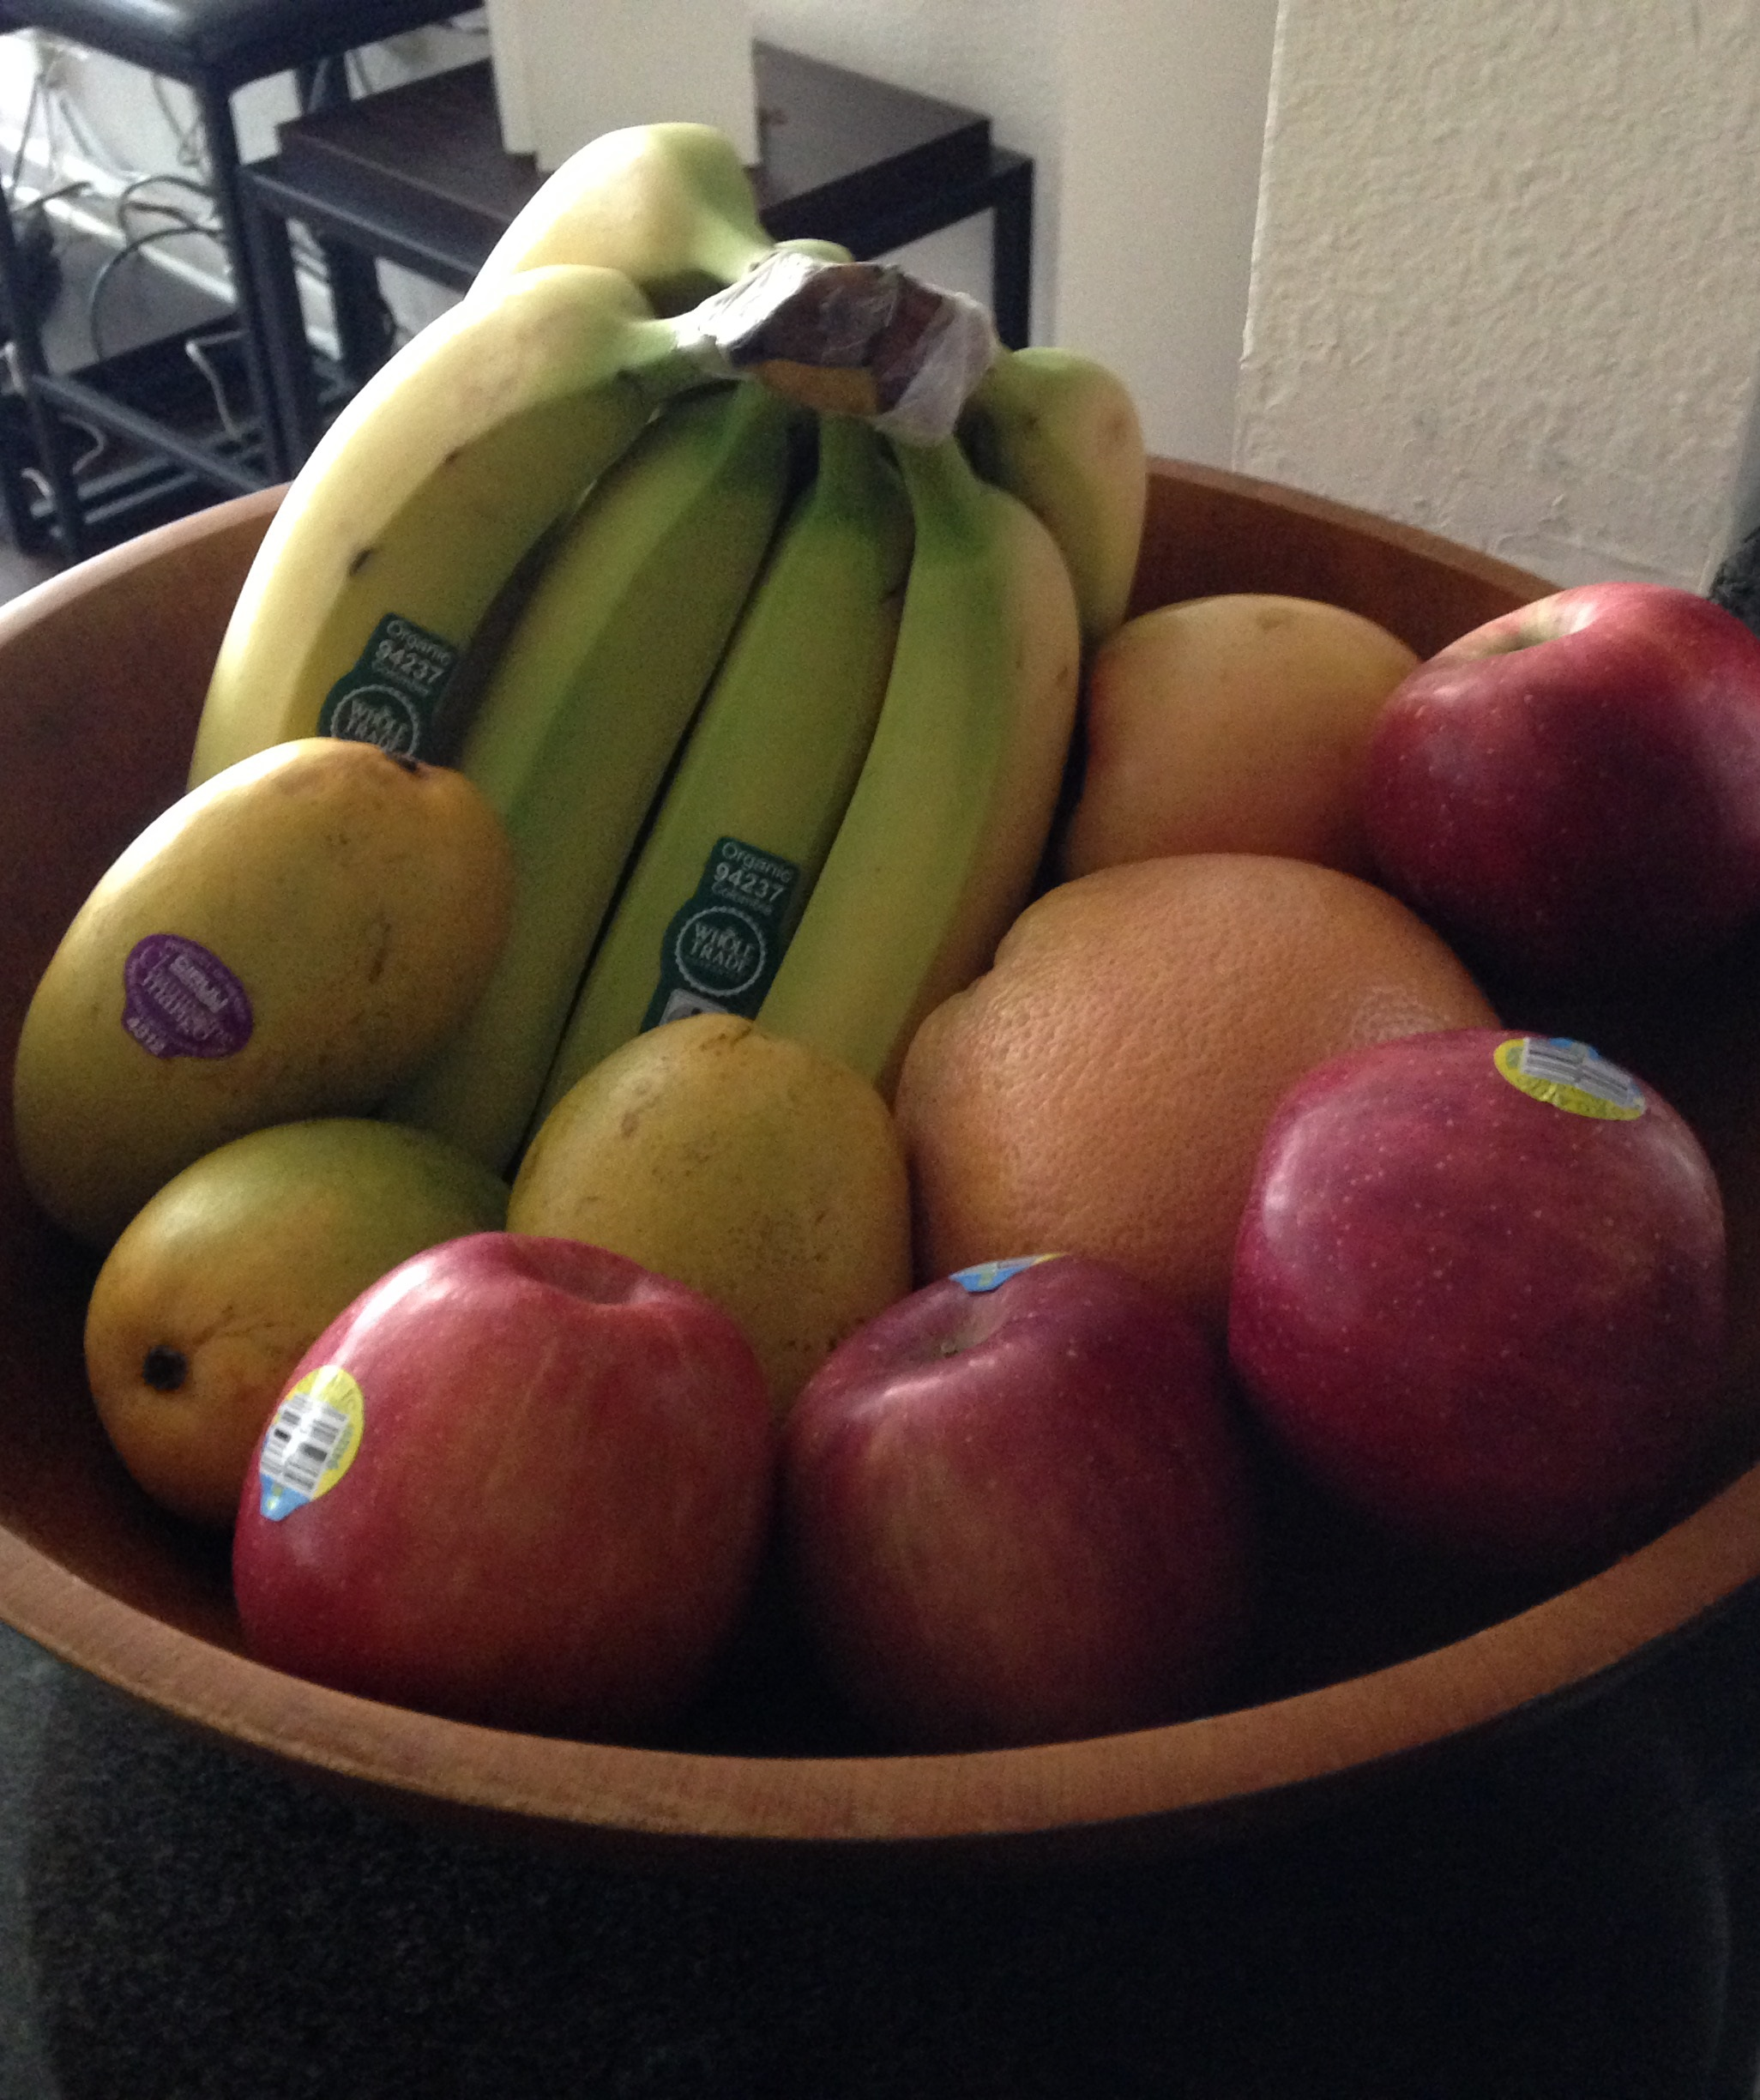
\includegraphics[height=\paperheight,
				keepaspectratio]{./Images/FruitBowl.jpg}}%
			\vfill
}}}

%STEAK
\newcommand\Steak{%
	\put(0,0){%
		\parbox[b][\paperheight]{\paperwidth}{%
			\vfill
			\centering
			{\transparent{0.3} 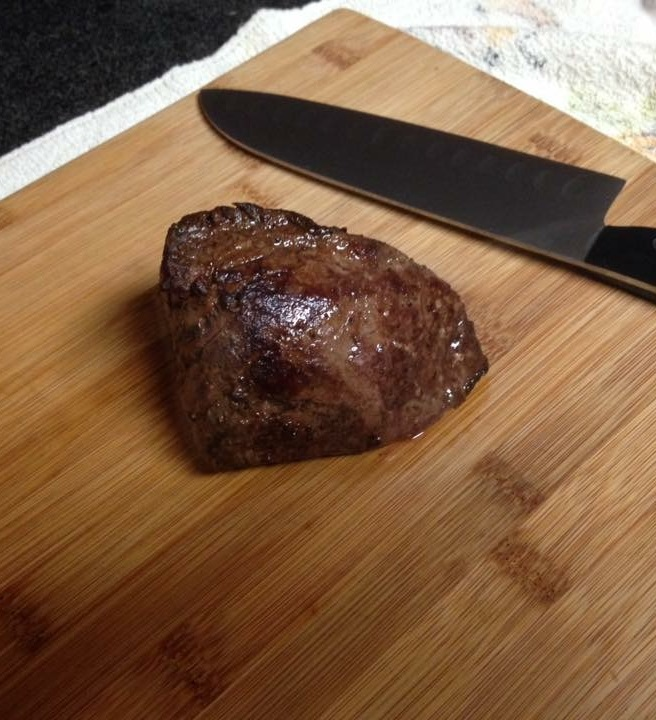
\includegraphics[height=\paperheight,
				keepaspectratio]{./Images/Steak.jpg}}%
			\vfill
}}}

%APPLETARTLARGE
\newcommand\AppleTartLarge{%
	\put(0,0){%
		\parbox[b][\paperheight]{\paperwidth}{%
			\vfill
			\centering
			{\transparent{0.3} 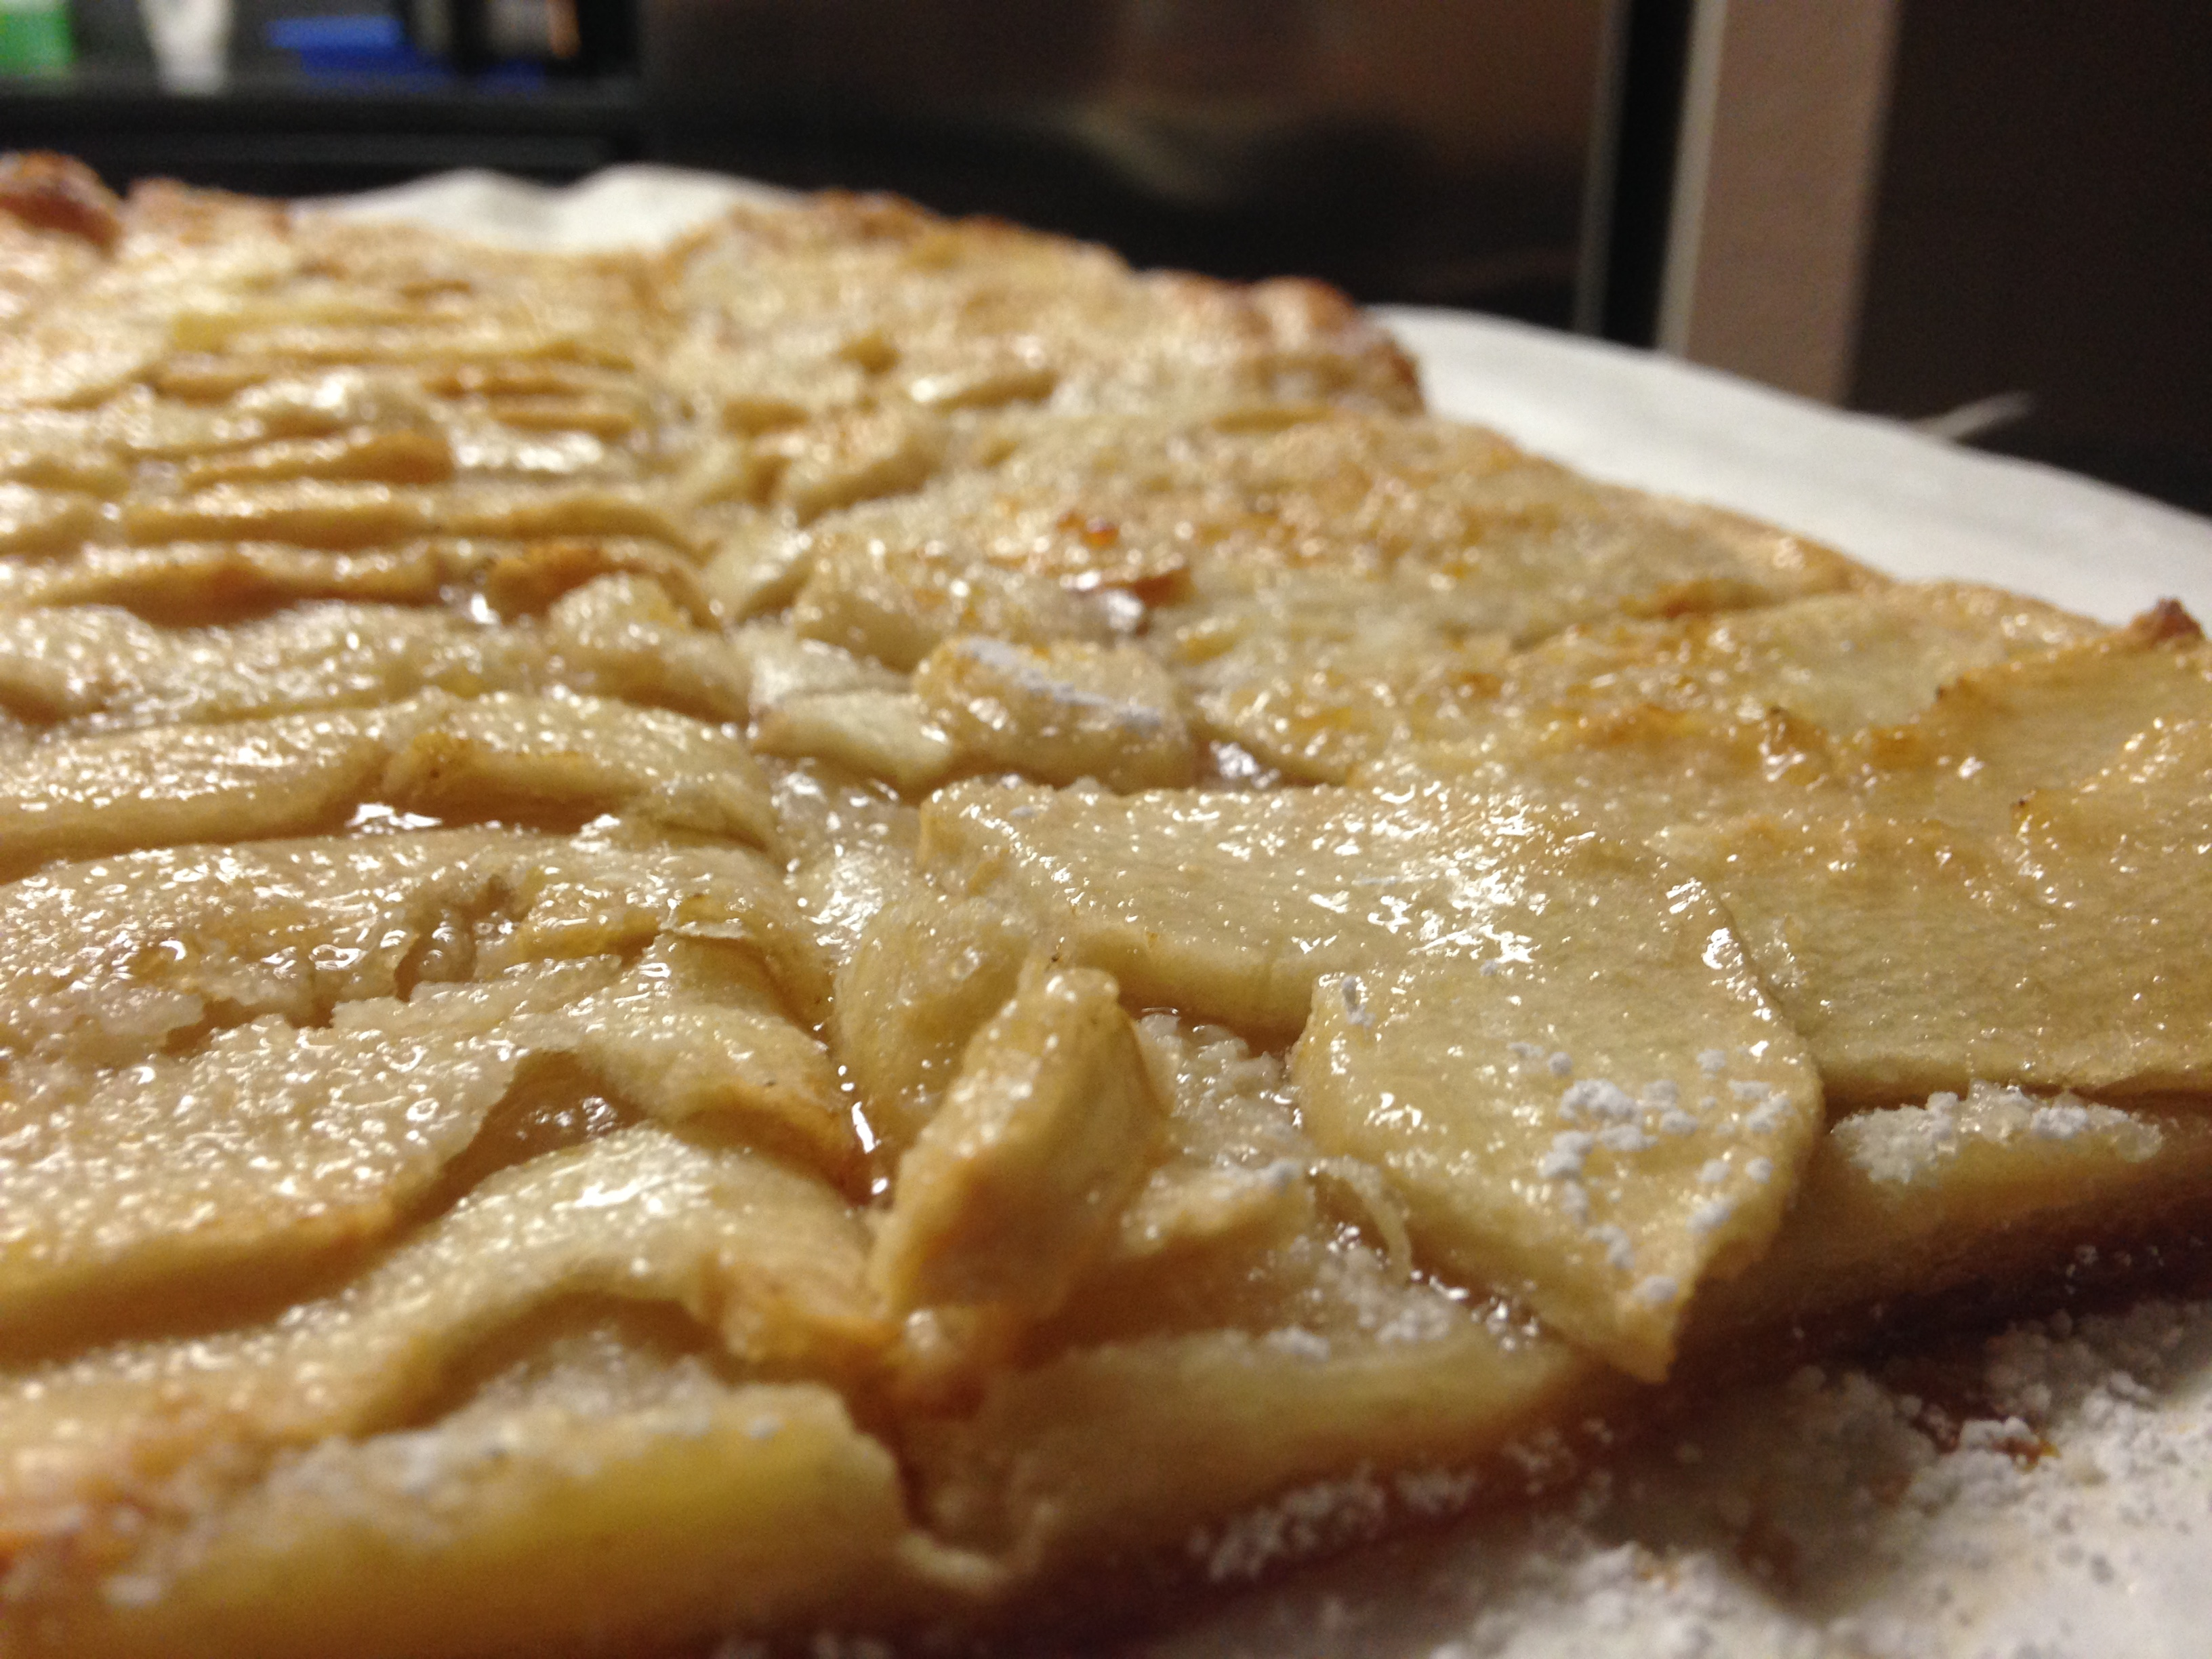
\includegraphics[height=\paperheight,
				keepaspectratio]{./Images/AppleTartLarge.jpg}}%
			\vfill
}}}

%STRAWBERRIES
\newcommand\Strawberries{%
	\put(0,0){%
		\parbox[b][\paperheight]{\paperwidth}{%
			\vfill
			\centering
			{\transparent{0.3} 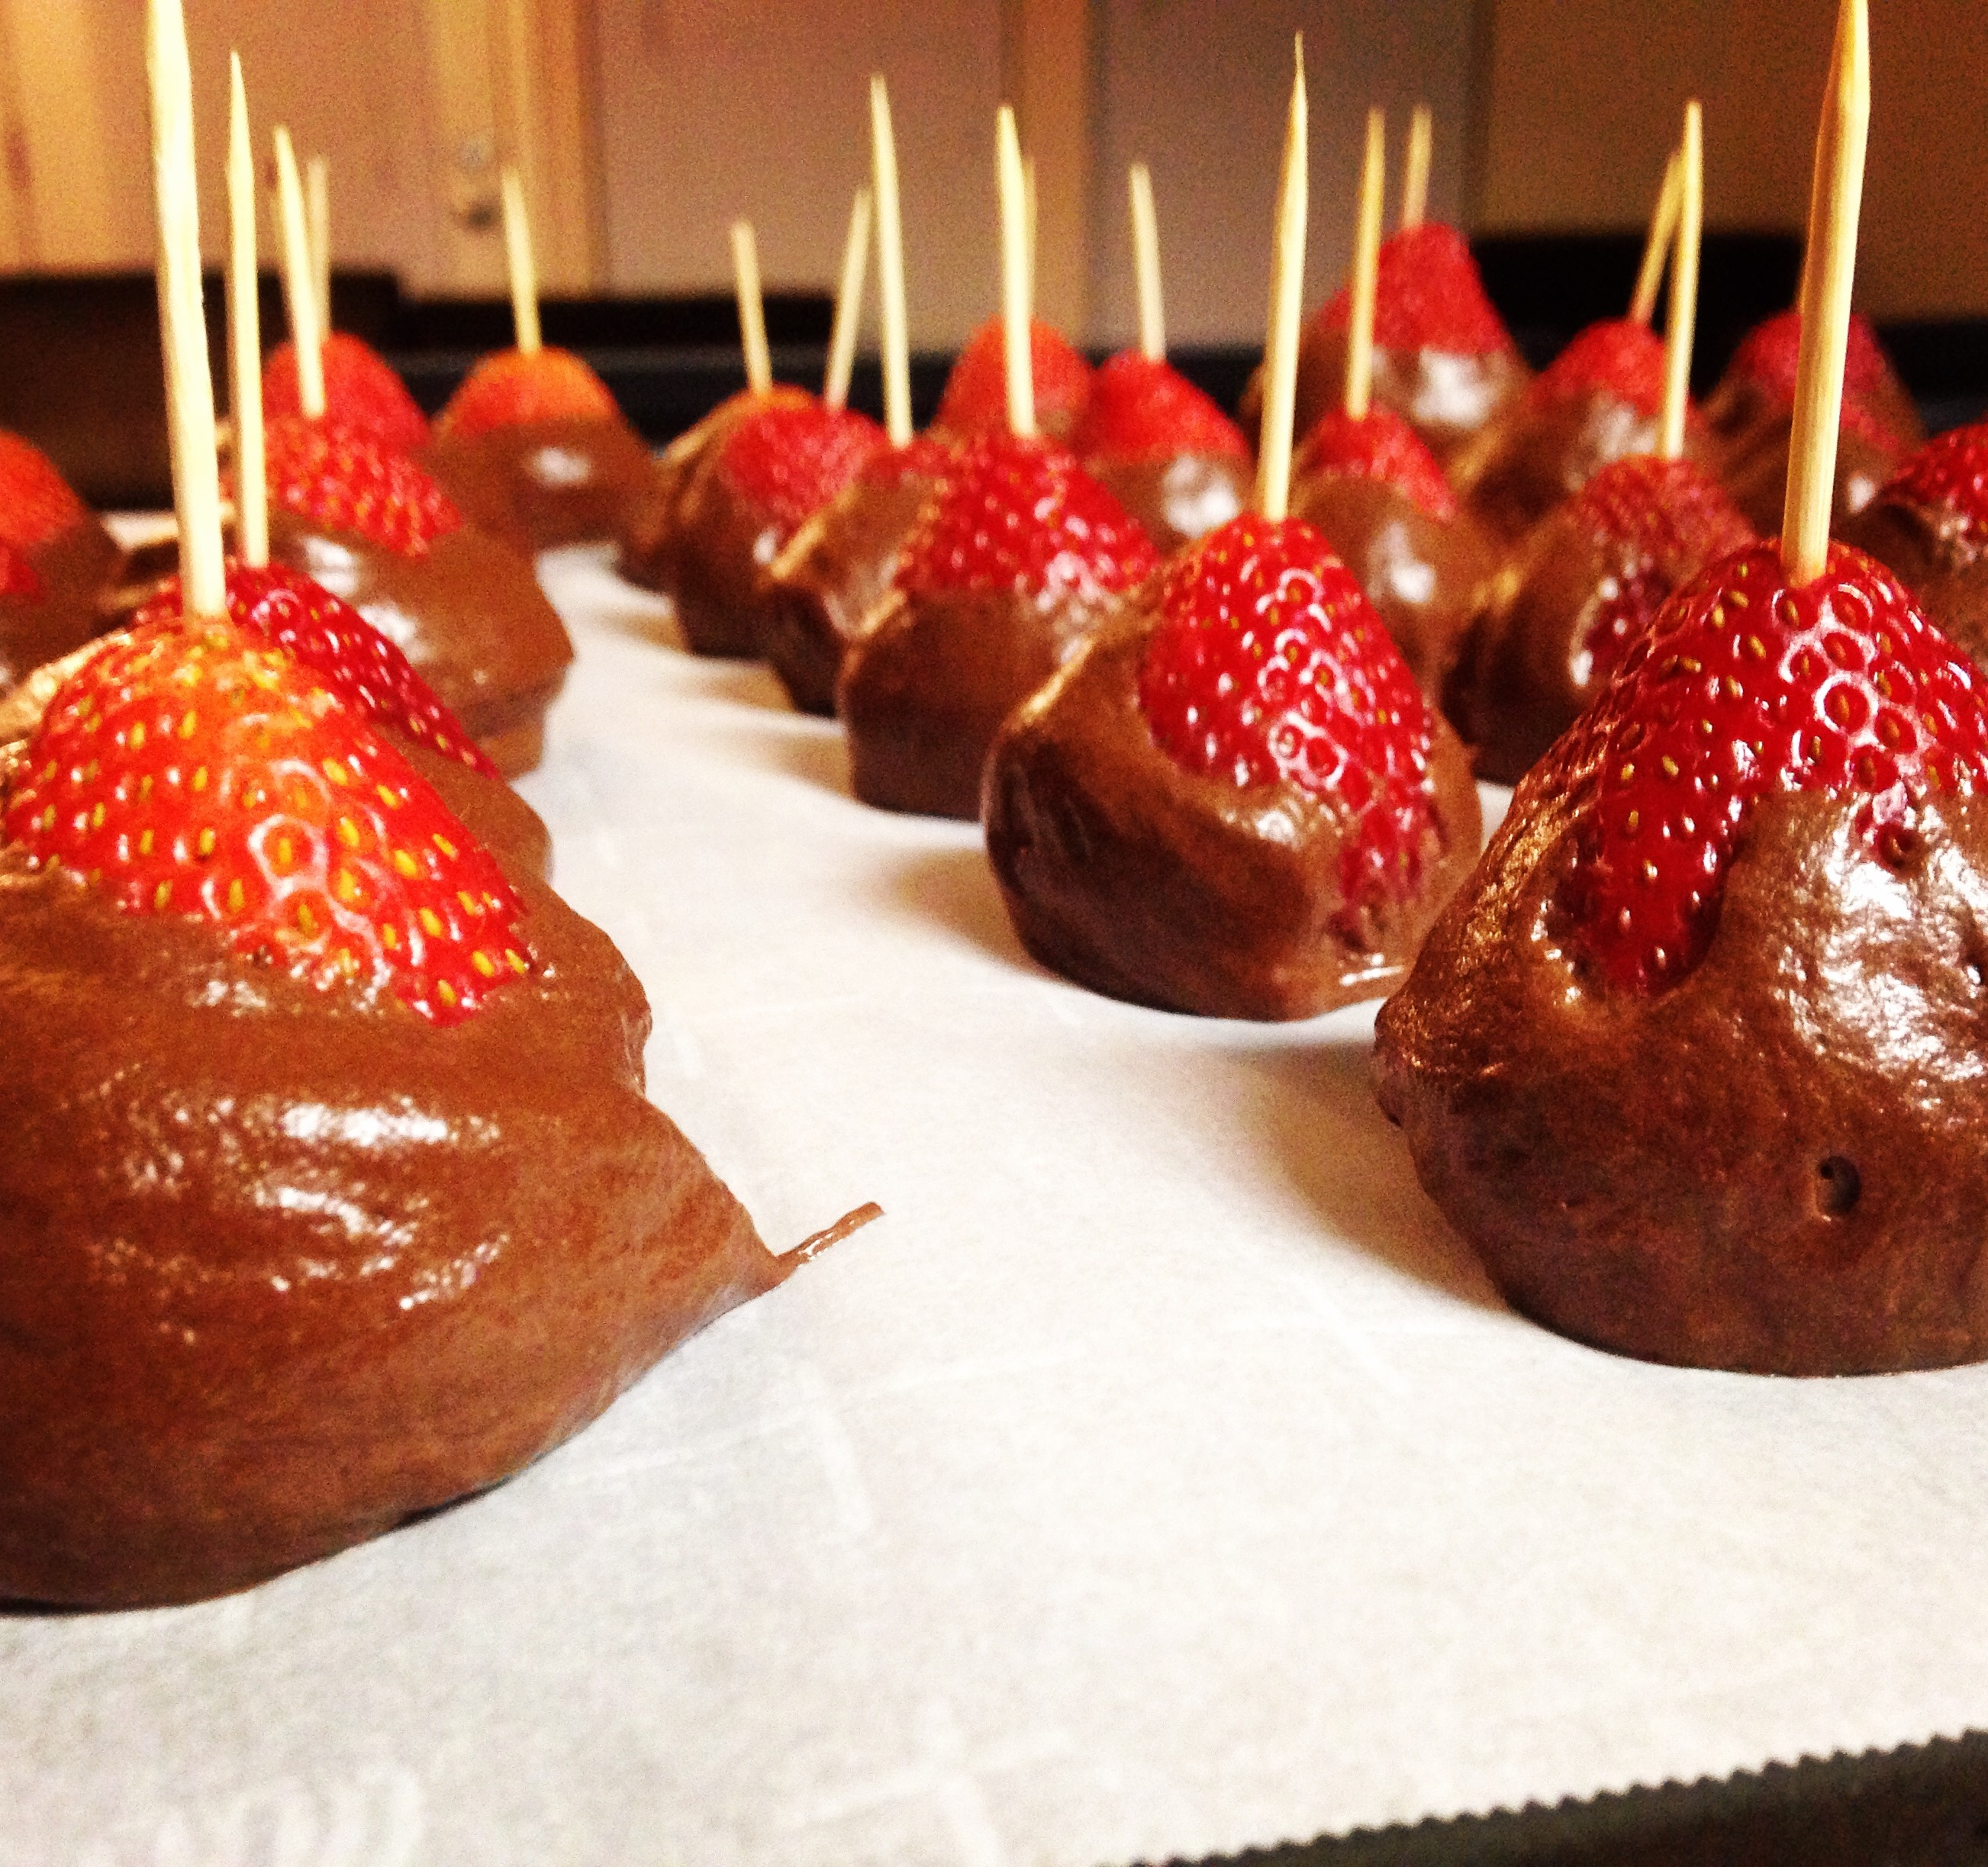
\includegraphics[height=\paperheight,%
				keepaspectratio]{./Images/Strawberries.jpg}}%
			\vfill
}}}

%SALMONVEGETABLERICE
\newcommand\SalmonVegetableRice{%
	\put(0,0){%
		\parbox[b][\paperheight]{\paperwidth}{%
			\vfill
			\centering
			{\transparent{0.3} 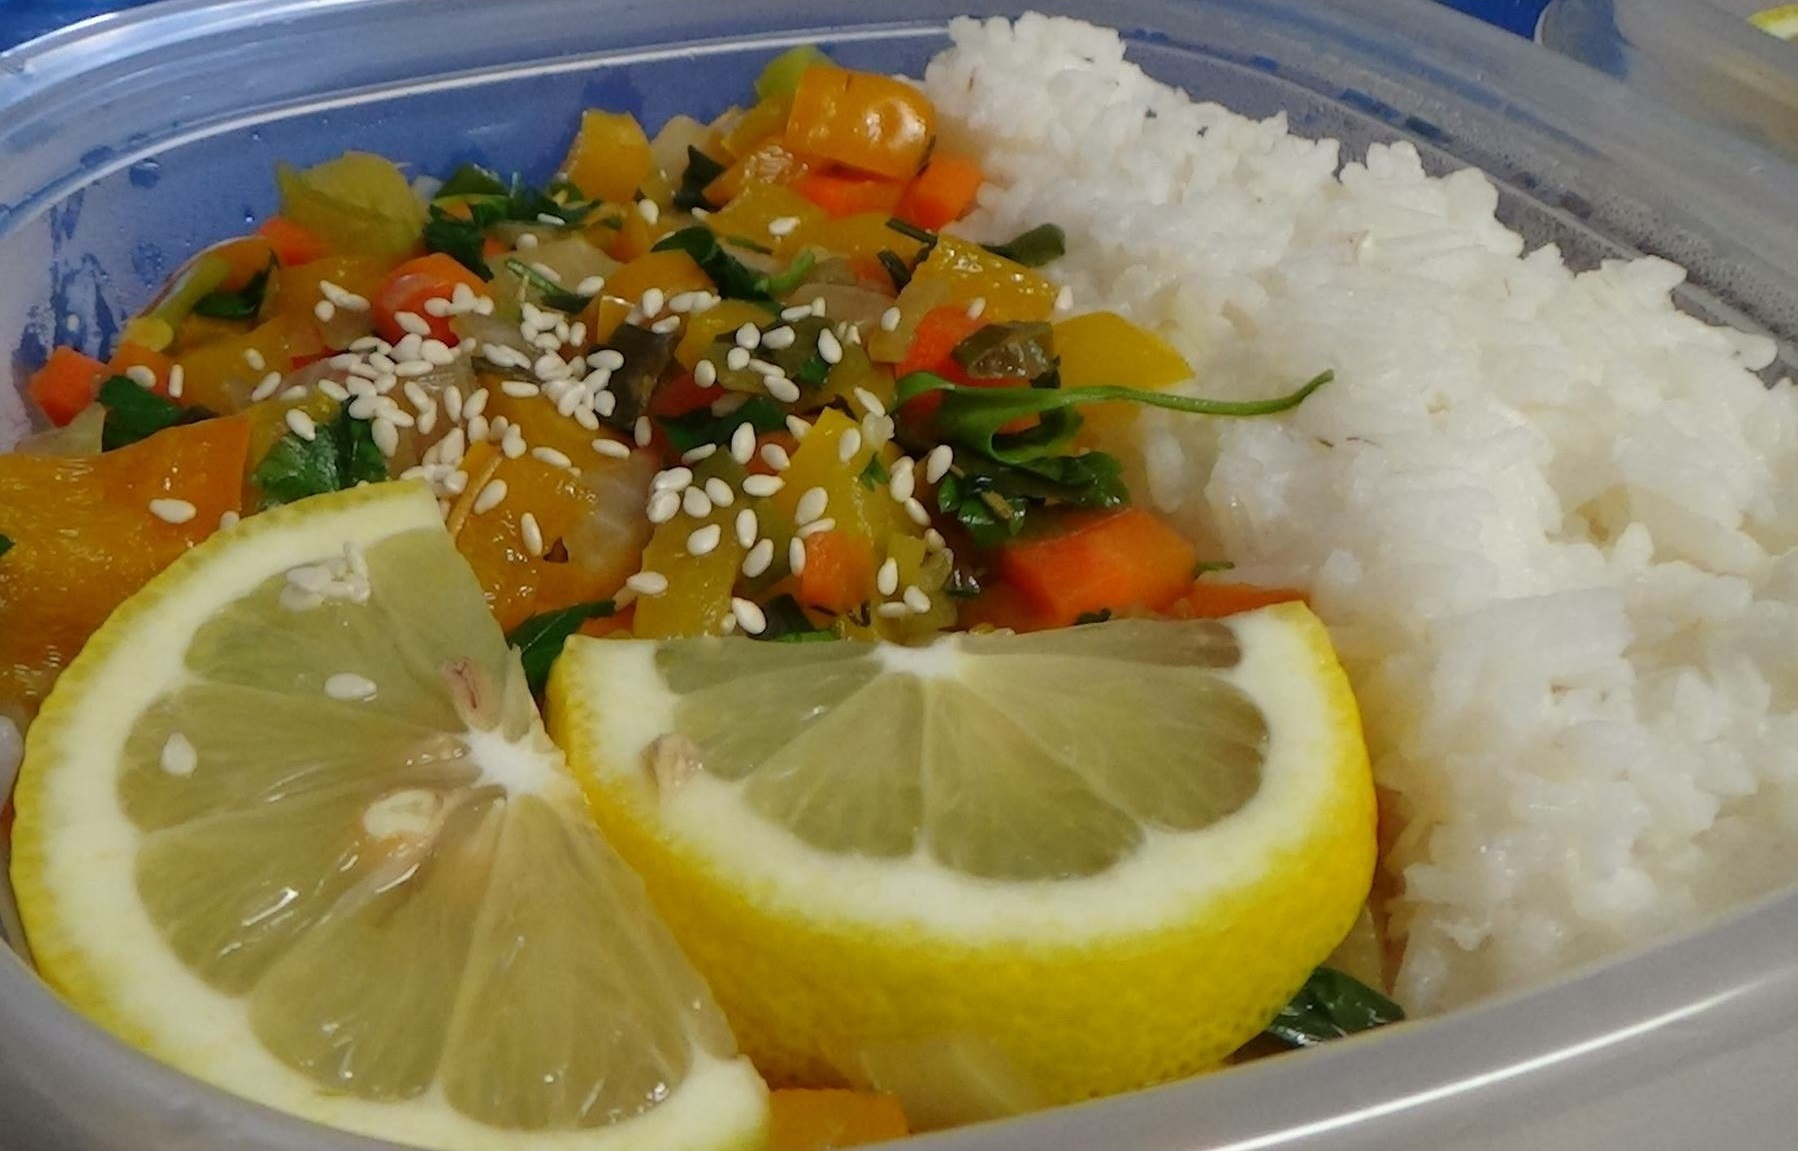
\includegraphics[height=\paperheight,%
				keepaspectratio]{./Images/SalmonVegetableRice.jpg}}%
			\vfill
}}}

%CHEESECAKE
\newcommand\Cheesecake{%
	\put(0,0){%
		\parbox[b][\paperheight]{\paperwidth}{%
			\vfill
			\centering
			{\transparent{0.3} 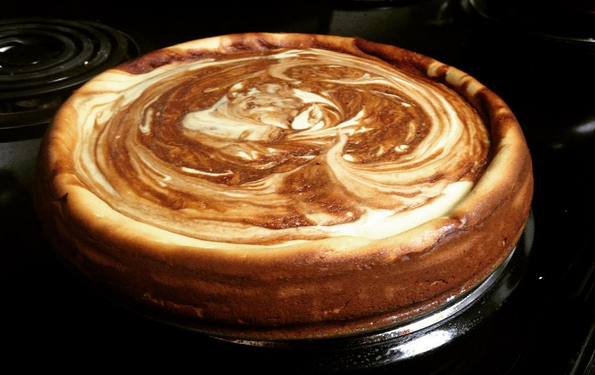
\includegraphics[height=\paperheight,%
				keepaspectratio]{./Images/MarbledCheesecake.png}}%
			\vfill
}}}

%CHICKENSALAD
\newcommand\ChickenSalad{%
	\put(0,0){%
		\parbox[b][\paperheight]{\paperwidth}{%
			\vfill
			\centering
			{\transparent{0.3} 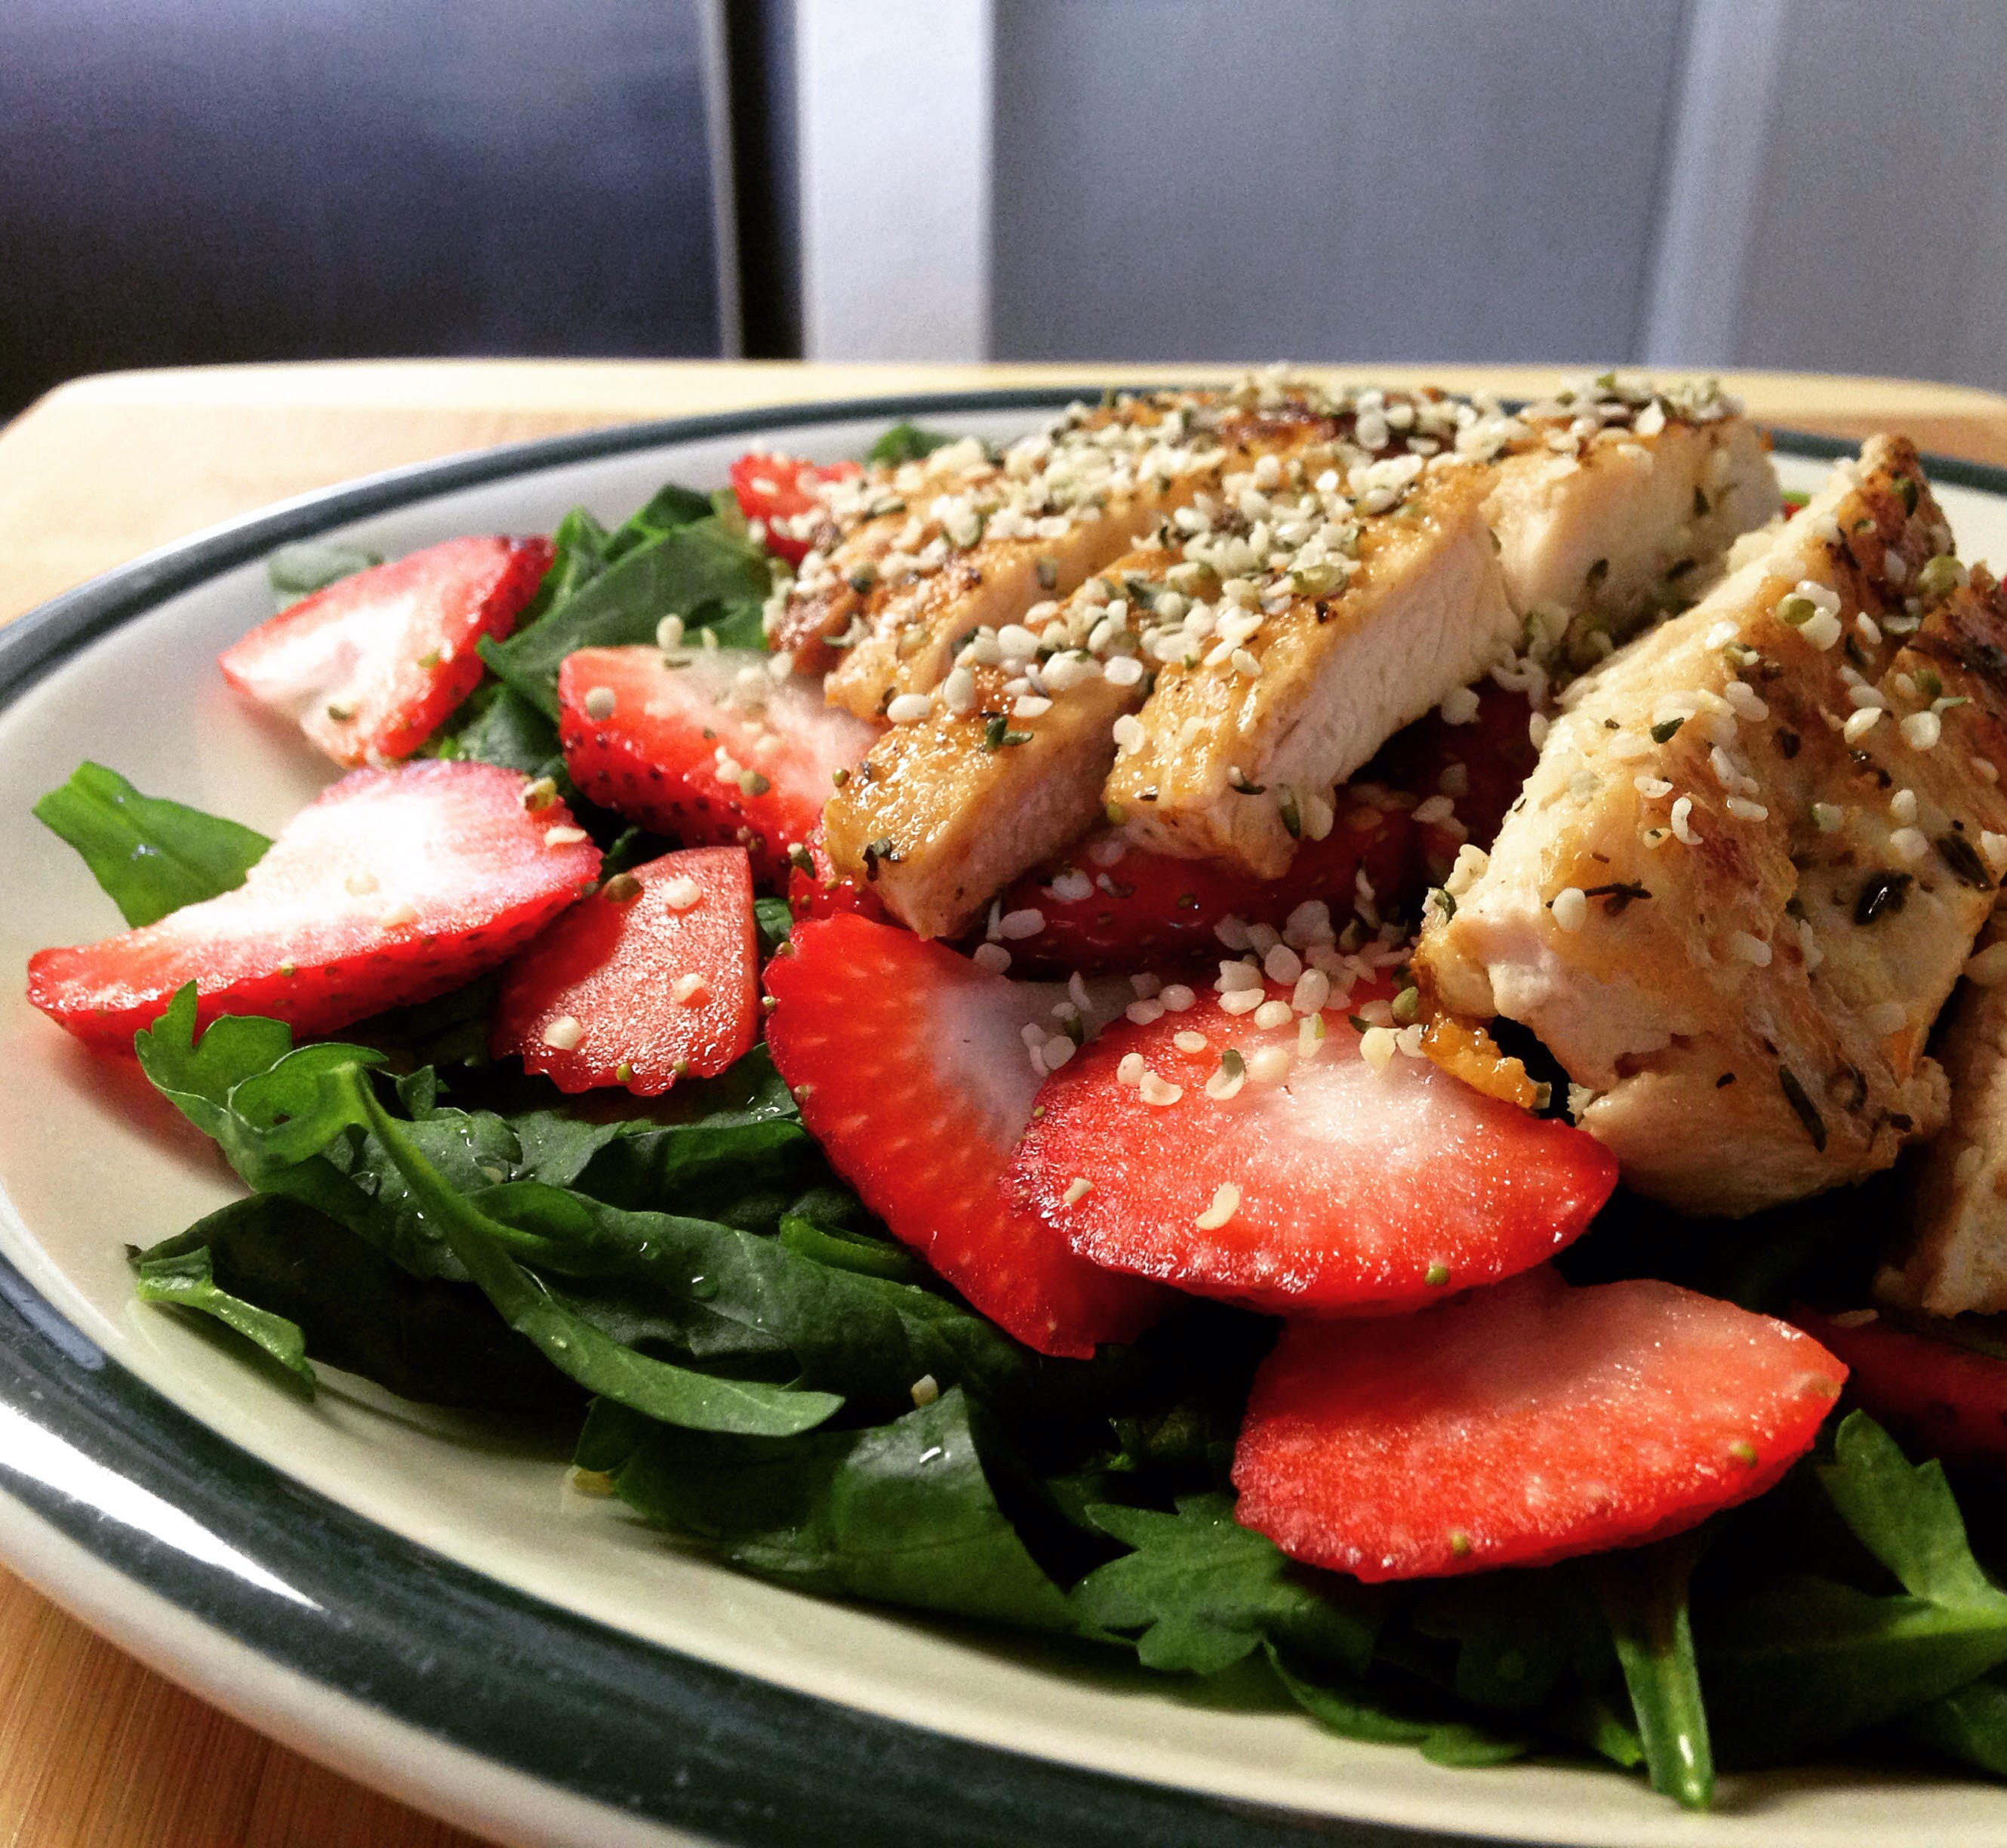
\includegraphics[height=\paperheight,%
				keepaspectratio]{./Images/ChickenSalad.jpg}}%
			\vfill
}}}

%MEXICANSOUP
\newcommand\MexicanSoup{%
	\put(0,0){%
		\parbox[b][\paperheight]{\paperwidth}{%
			\vfill
			\centering
			{\transparent{0.3} 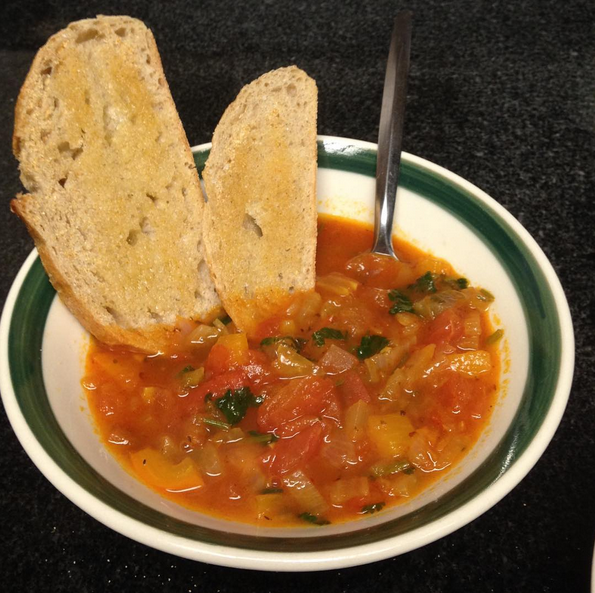
\includegraphics[height=\paperheight,%
				keepaspectratio]{./Images/SpicyMexicanSoup.png}}%
			\vfill
}}}

%CALZONE
\newcommand\Calzone{%
	\put(0,0){%
		\parbox[b][\paperheight]{\paperwidth}{%
			\vfill
			\centering
			{\transparent{0.3} 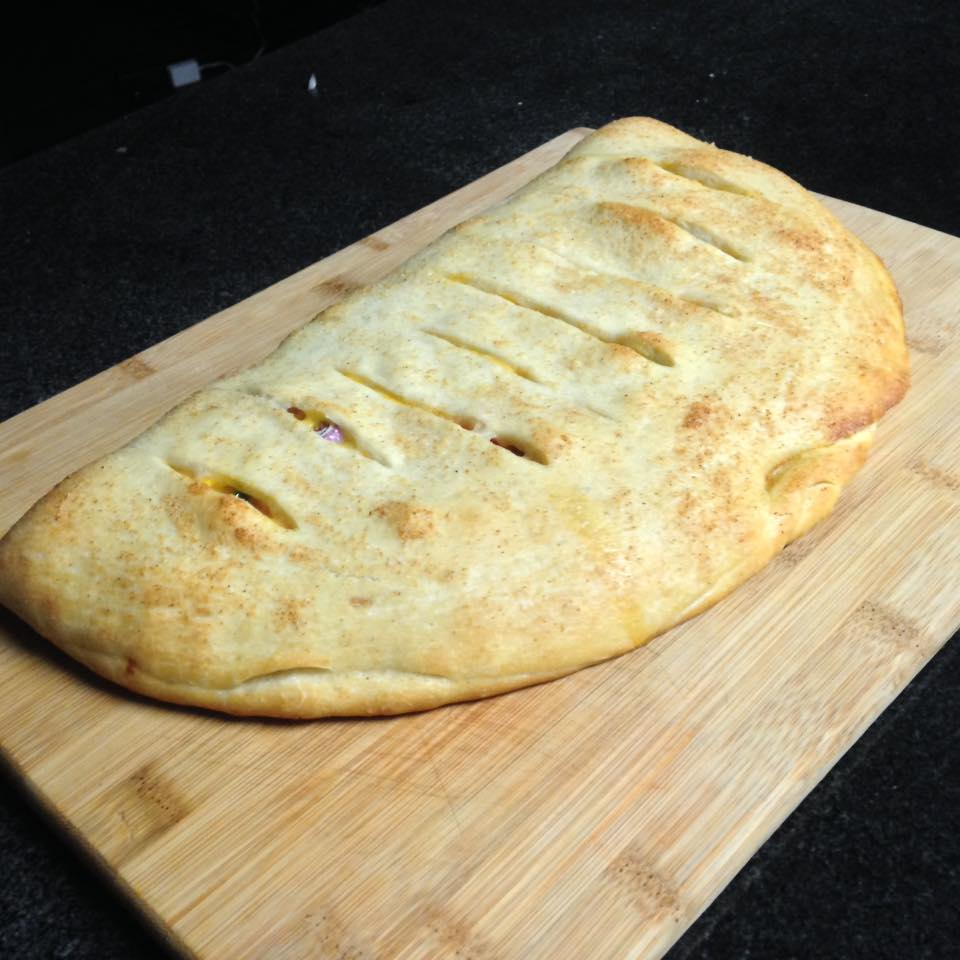
\includegraphics[height=\paperheight,%
				keepaspectratio]{./Images/Calzone.jpg}}%
			\vfill
}}}

%CHEESECAKETOPPING
\newcommand\CheesecakeTopping{%
	\put(0,0){%
		\parbox[b][\paperheight]{\paperwidth}{%
			\vfill
			\centering
			{\transparent{0.3} 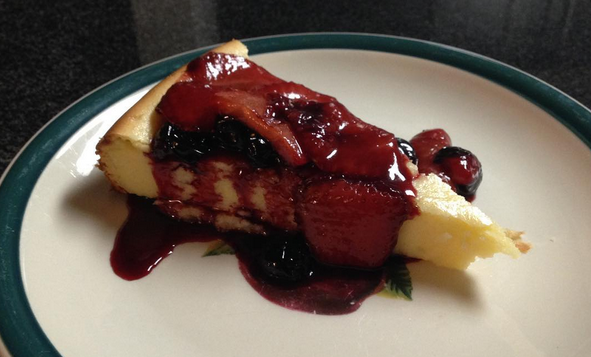
\includegraphics[height=\paperheight,%
				keepaspectratio]{./Images/CheesecakeTopping.png}}%
			\vfill
}}}

%MANGOSALSATACO
\newcommand\MangoSalsaTaco{%
	\put(0,0){%
		\parbox[b][\paperheight]{\paperwidth}{%
			\vfill
			\centering
			{\transparent{0.3} 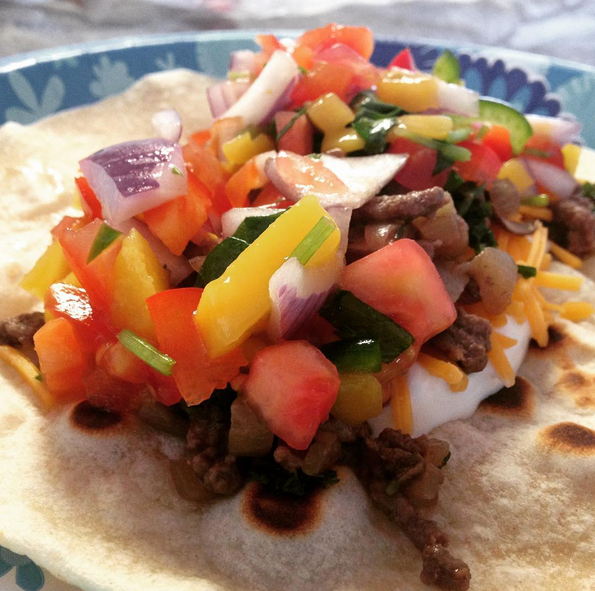
\includegraphics[height=\paperheight,%
				keepaspectratio]{./Images/MangeSalsaTacos.png}}%
			\vfill
}}}

%EGGSANDWICH
\newcommand\EggSandwich{%
	\put(0,0){%
		\parbox[b][\paperheight]{\paperwidth}{%
			\vfill
			\centering
			{\transparent{0.3} 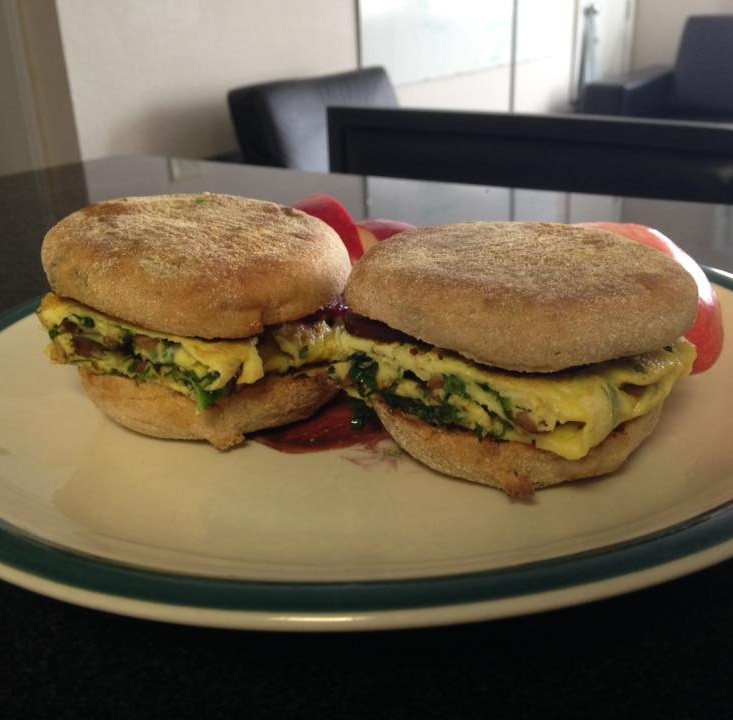
\includegraphics[height=\paperheight,%
				keepaspectratio]{./Images/EggSandwich.jpg}}%
			\vfill
}}}

%APPLETART
\newcommand\AppleTart{%
	\put(0,0){%
		\parbox[b][\paperheight]{\paperwidth}{%
			\vfill
			\centering
			{\transparent{0.3} 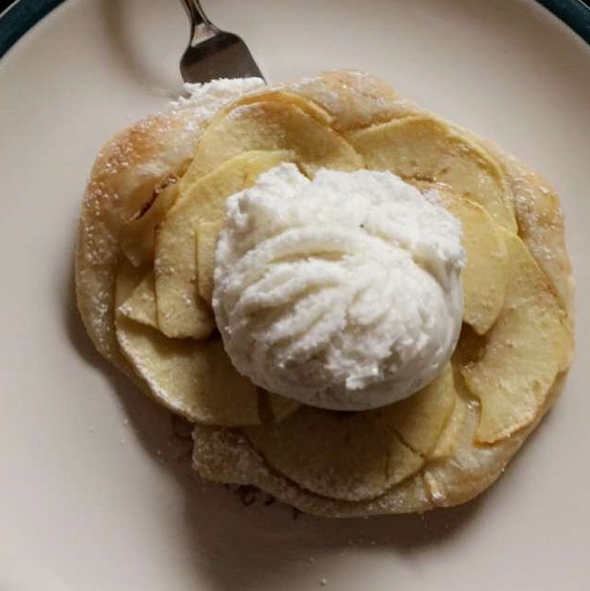
\includegraphics[height=\paperheight,%
				keepaspectratio]{./Images/AppleTartDesert.png}}%
			\vfill
}}}

%MARINATEDCHICKENANDRICE
\newcommand\MarinatedChickenAndRice{%
	\put(0,0){%
		\parbox[b][\paperheight]{\paperwidth}{%
			\vfill
			\centering
			{\transparent{0.3} 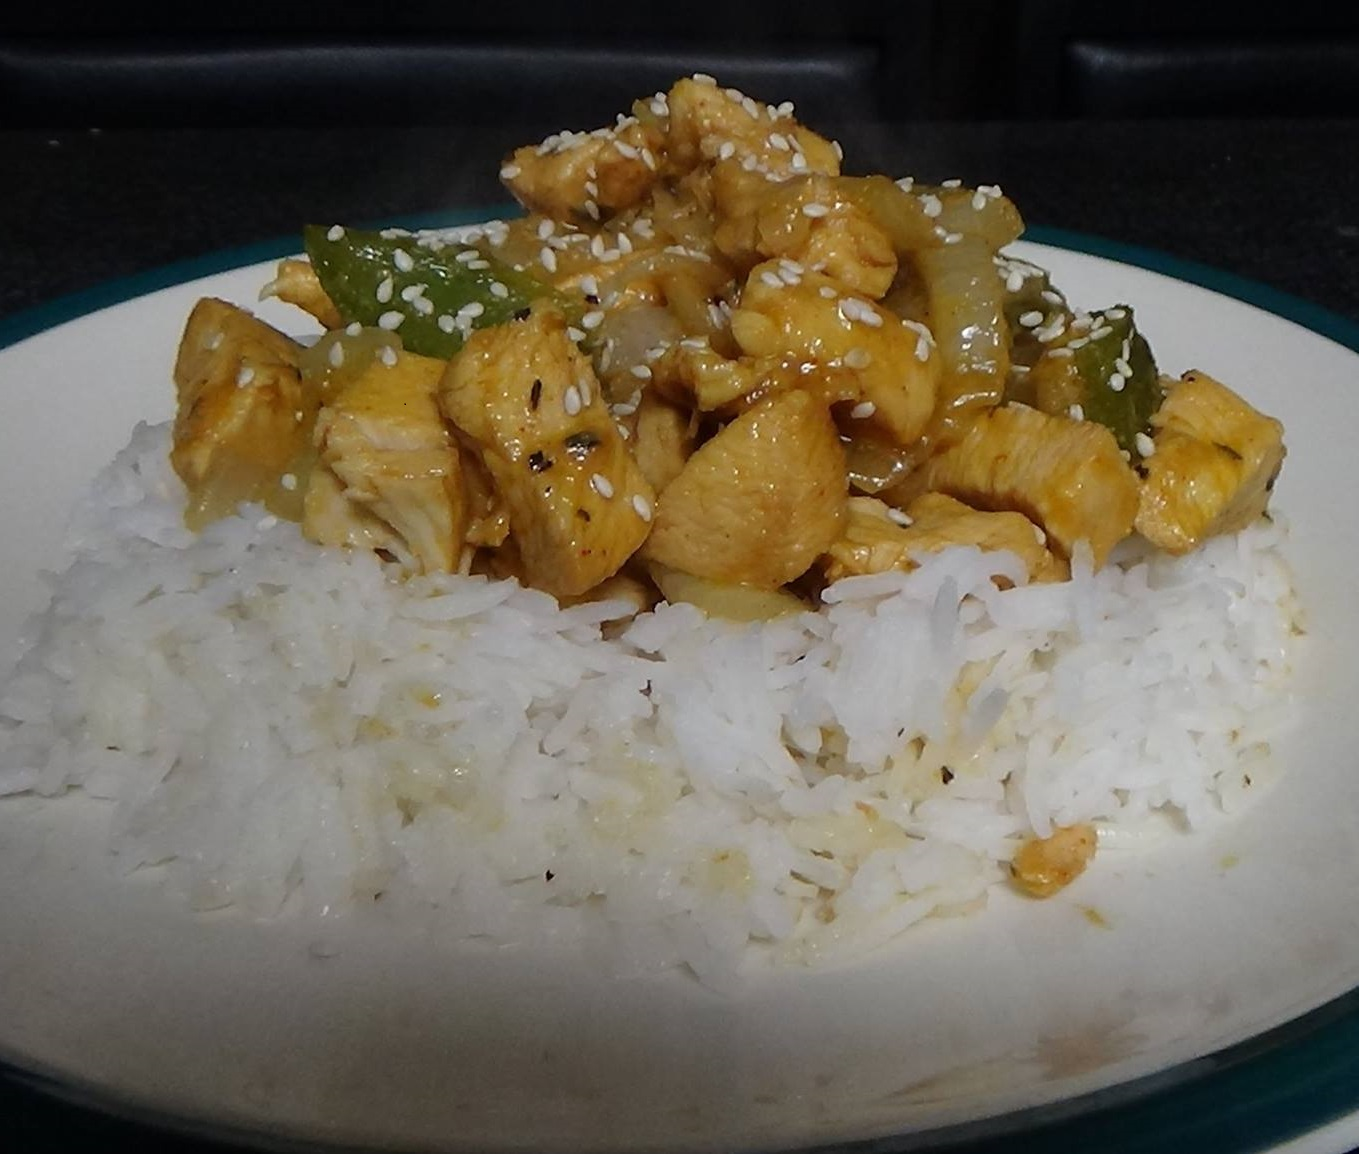
\includegraphics[height=\paperheight,%
				keepaspectratio]{./Images/chickenveggiesrice.jpg}}%
			\vfill
}}}

%FETASPINACHEGGS
\newcommand\FetaSpinachEggs{%
	\put(0,0){%
		\parbox[b][\paperheight]{\paperwidth}{%
			\vfill
			\centering
			{\transparent{0.3} 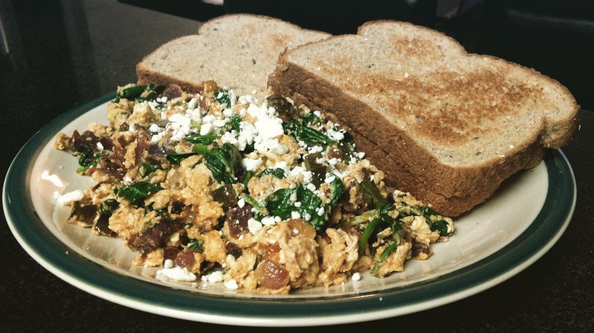
\includegraphics[height=\paperheight,%
				keepaspectratio]{./Images/FetaAndSpinachScrambledEggs.png}}%
			\vfill
}}}

%STIRFRYRICENOODLES
\newcommand\StirFryRiceNoodles{%
	\put(0,0){%
		\parbox[b][\paperheight]{\paperwidth}{%
			\vfill
			\centering
			{\transparent{0.3} 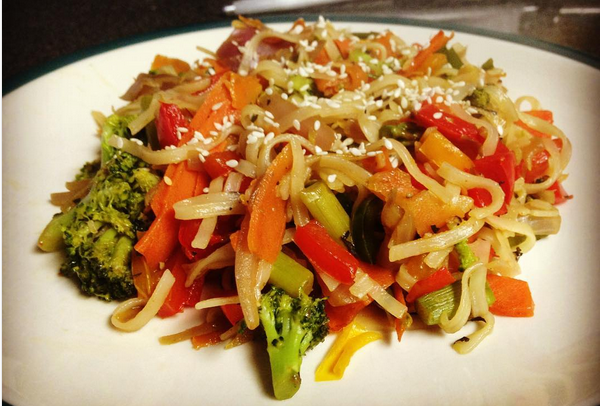
\includegraphics[height=\paperheight,%
				keepaspectratio]{./Images/StirFry_RiceNoodles.png}}%
			\vfill
}}}

%ALFREDO
\newcommand\Alfredo{%
	\put(0,0){%
		\parbox[b][\paperheight]{\paperwidth}{%
			\vfill
			\centering
			{\transparent{0.3} 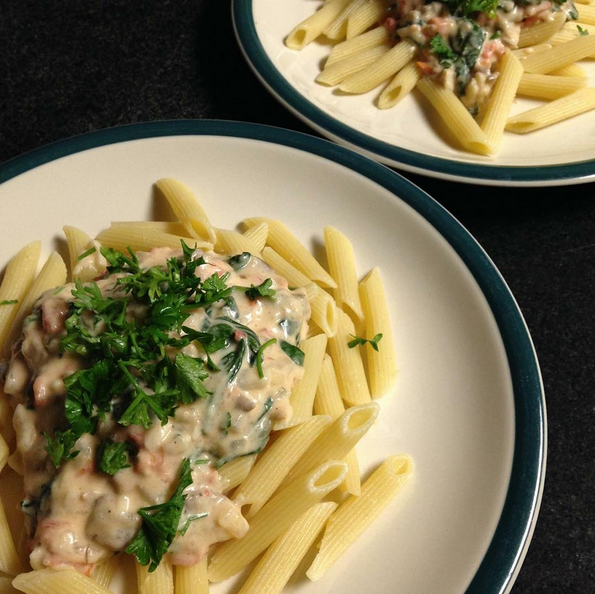
\includegraphics[height=\paperheight,%
				keepaspectratio]{./Images/Alfredo.png}}%
			\vfill
}}}

%STEAKANDEGGS
\newcommand\SteakAndEggs{%
	\put(0,0){%
		\parbox[b][\paperheight]{\paperwidth}{%
			\vfill
			\centering
			{\transparent{0.3} 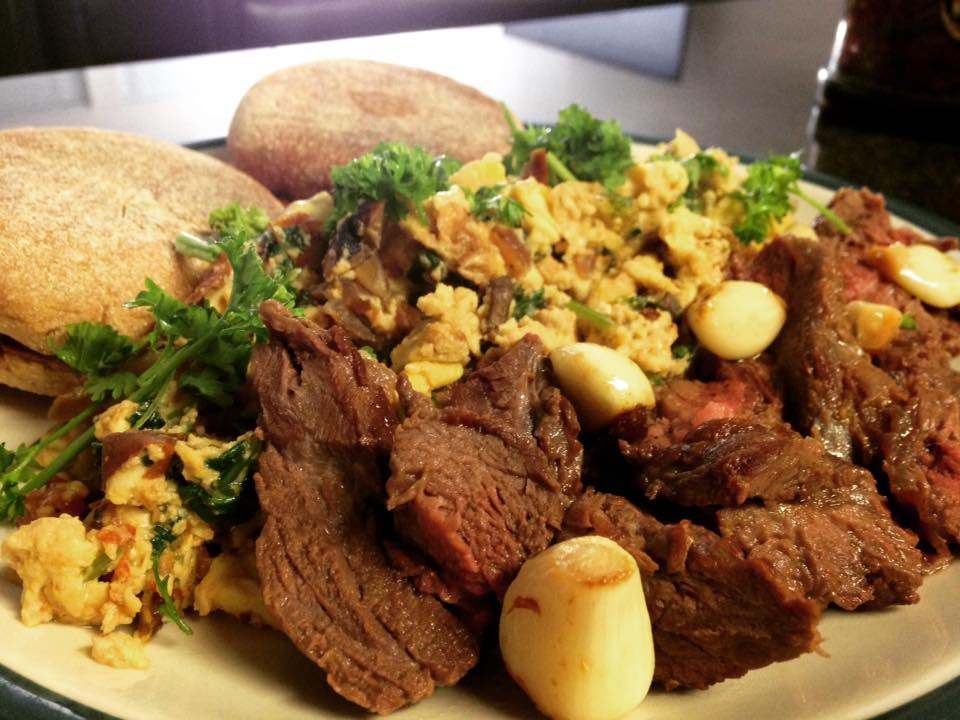
\includegraphics[height=\paperheight,%
				keepaspectratio]{./Images/SteakAndEggs.jpg}}%
			\vfill
}}}

%STEAKSANDWICH
\newcommand\SteakSandwich{%
	\put(0,0){%
		\parbox[b][\paperheight]{\paperwidth}{%
			\vfill
			\centering
			{\transparent{0.3} 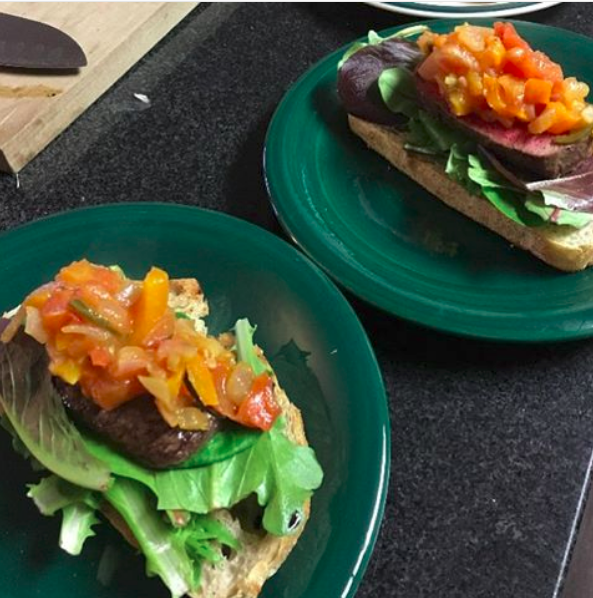
\includegraphics[height=\paperheight,%
				keepaspectratio]{./Images/SteakSandwich.png}}%
			\vfill
}}}

%PIZZA
\newcommand\Pizza{%
	\put(0,0){%
		\parbox[b][\paperheight]{\paperwidth}{%
			\vfill
			\centering
			{\transparent{0.3} 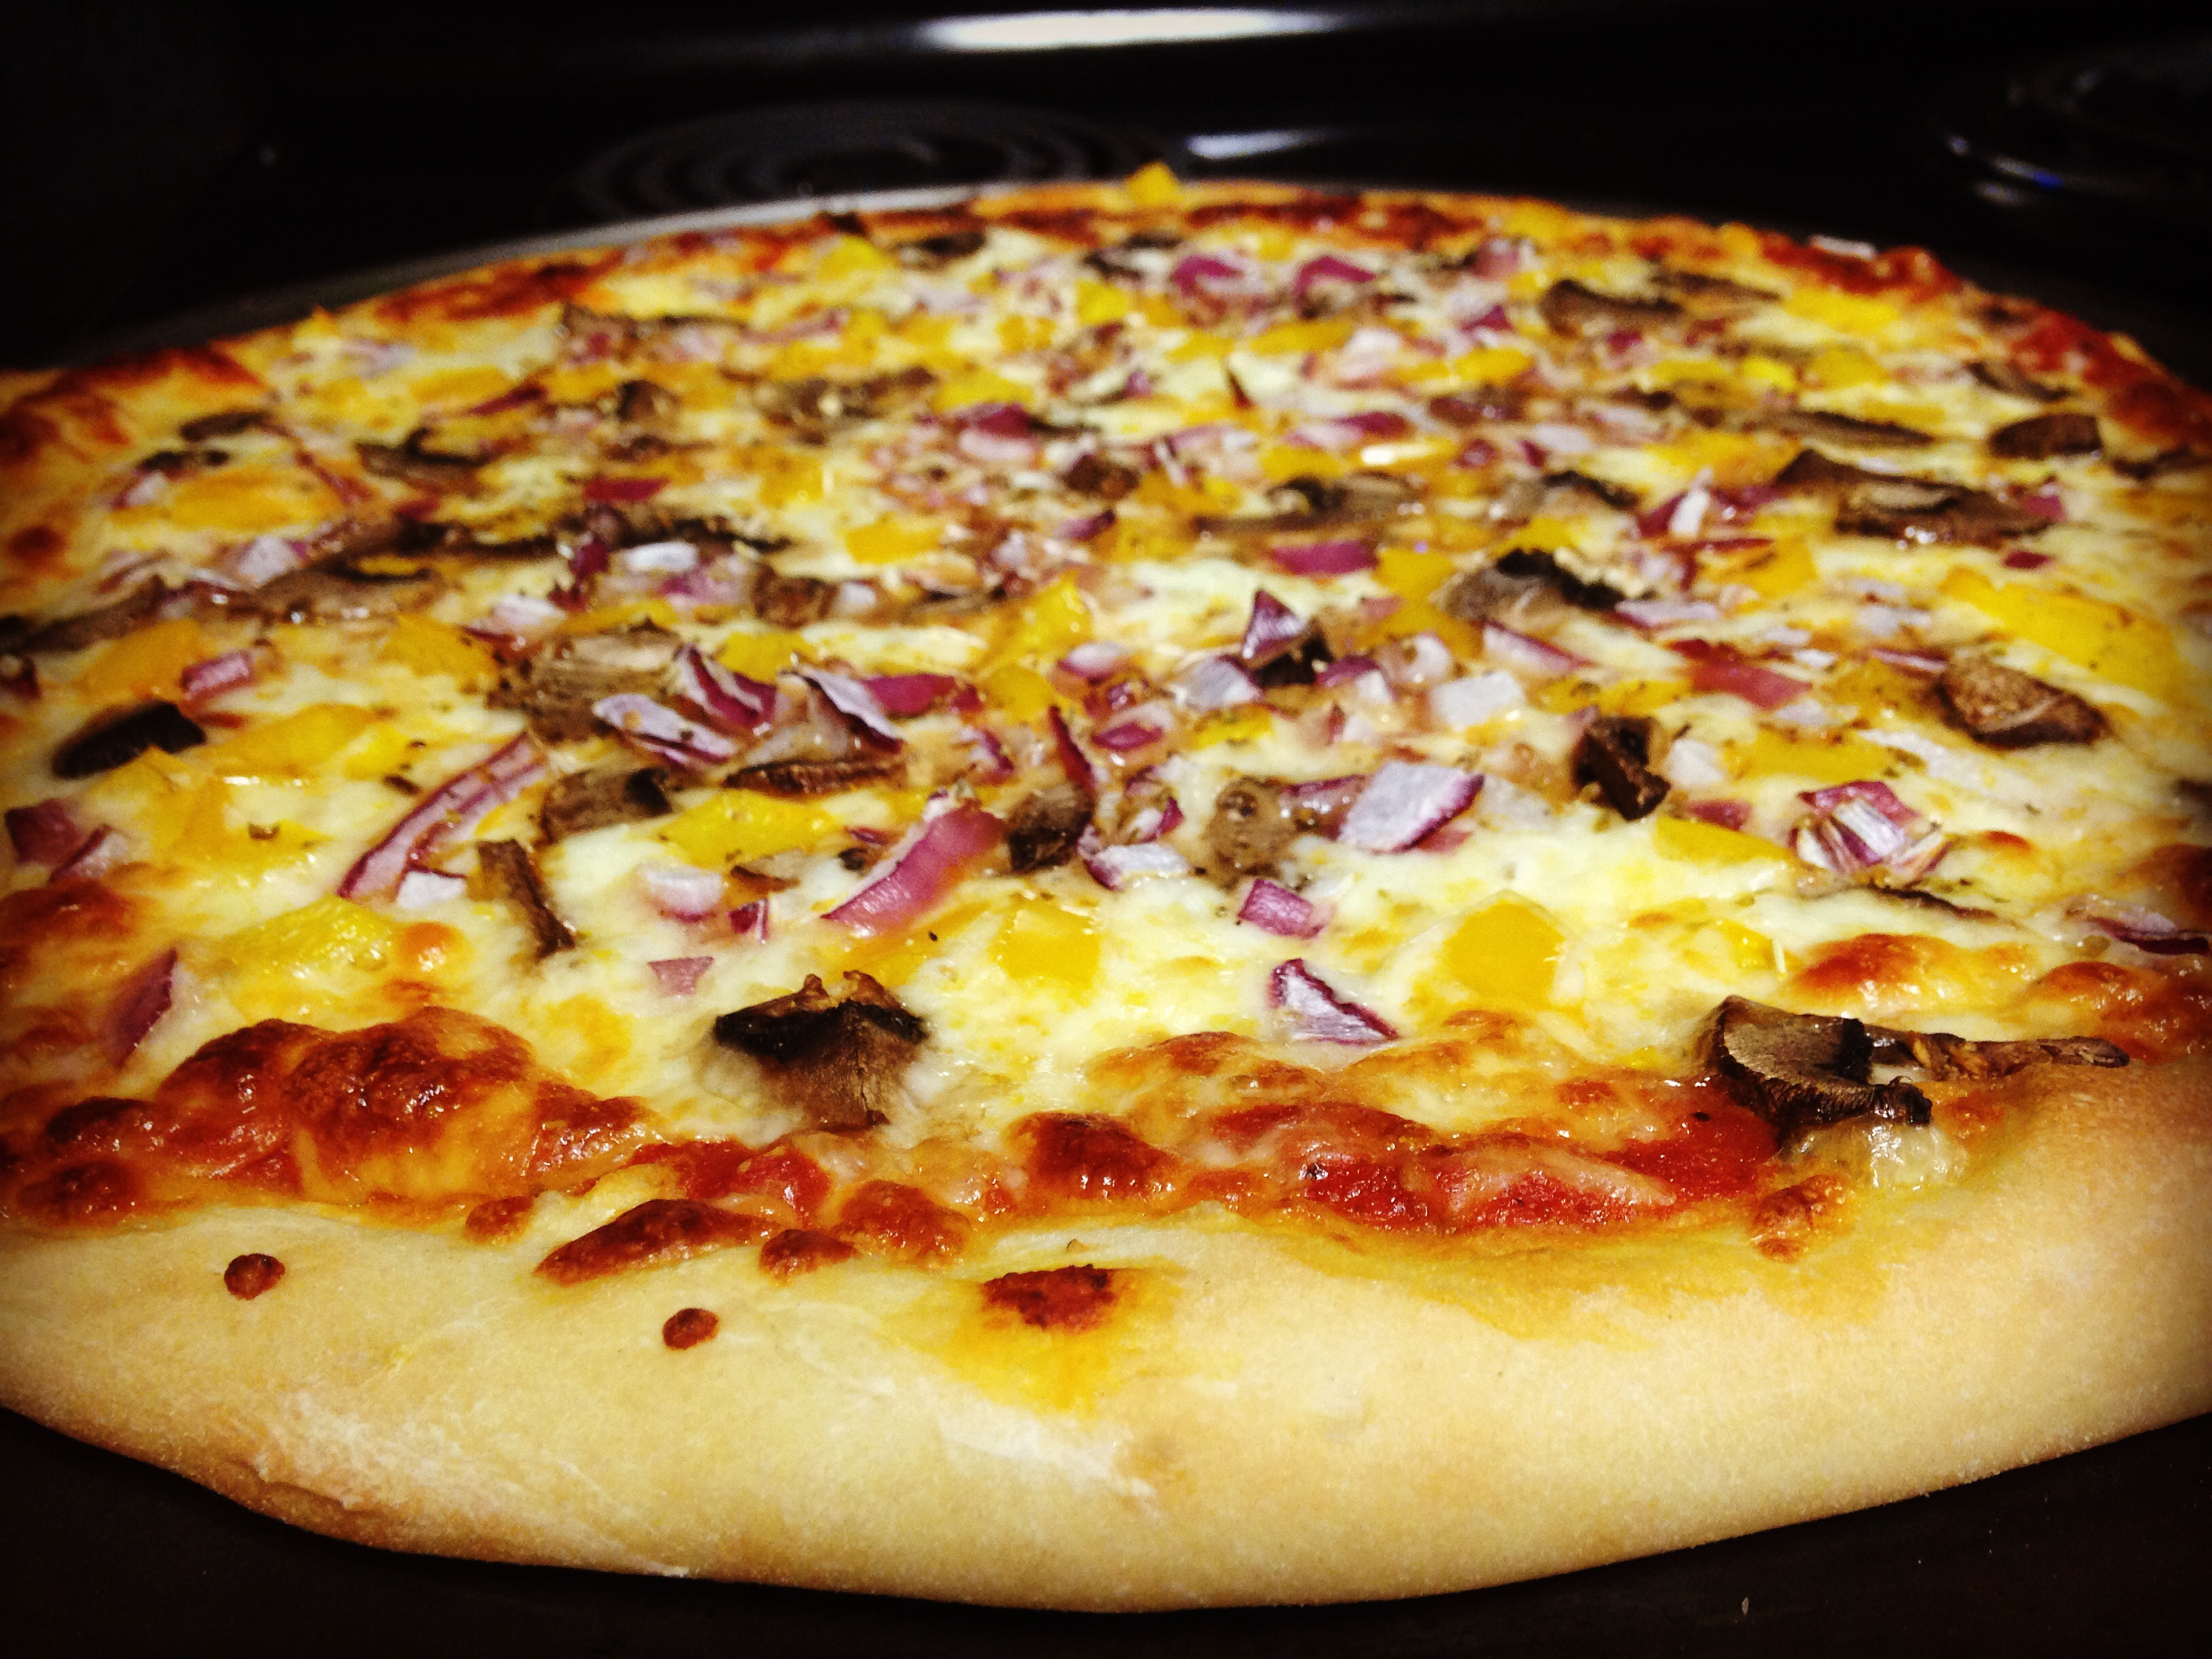
\includegraphics[height=\paperheight,%
				keepaspectratio]{./Images/Pizza.jpg}}%
			\vfill
}}}

%LASAGNA
\newcommand\Lasagna{%
	\put(0,0){%
		\parbox[b][\paperheight]{\paperwidth}{%
			\vfill
			\centering
			{\transparent{0.3} 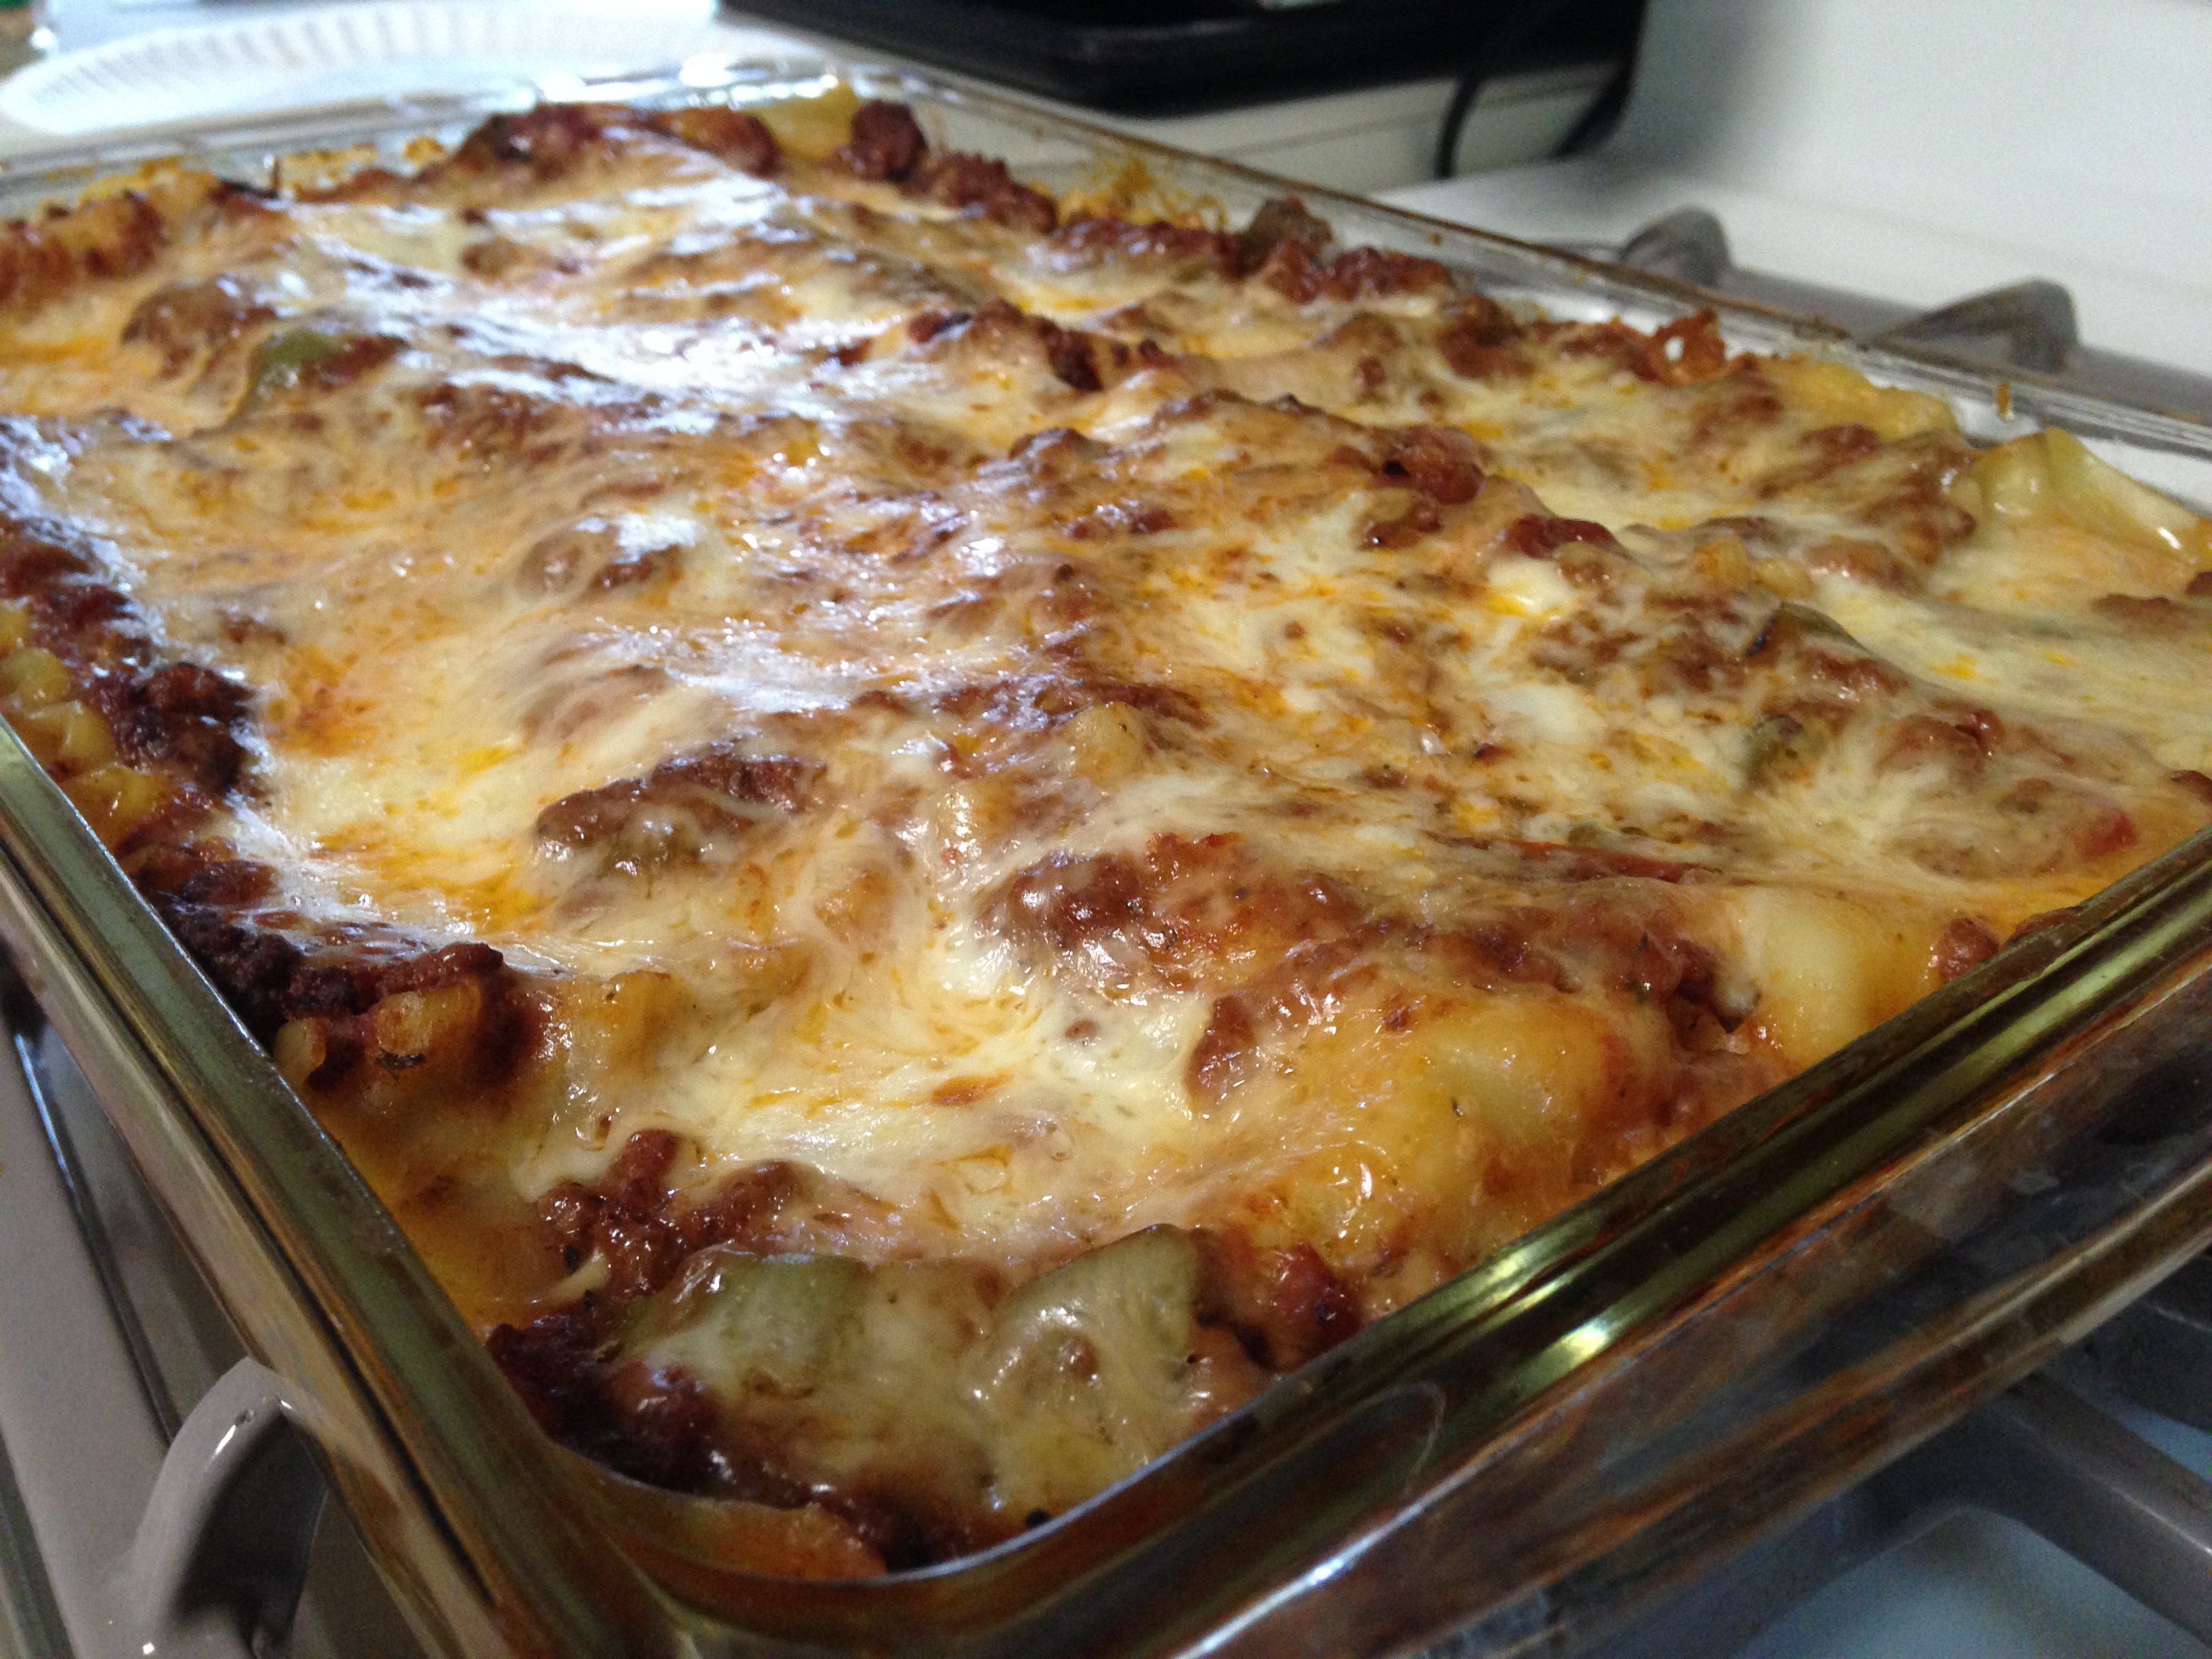
\includegraphics[height=\paperheight,%
				keepaspectratio]{./Images/Lasagna.jpg}}%
			\vfill
}}}

%VENISONBBQ
\newcommand\VenisonBBQ{%
	\put(0,0){%
		\parbox[b][\paperheight]{\paperwidth}{%
			\vfill
			\centering
			{\transparent{0.3} 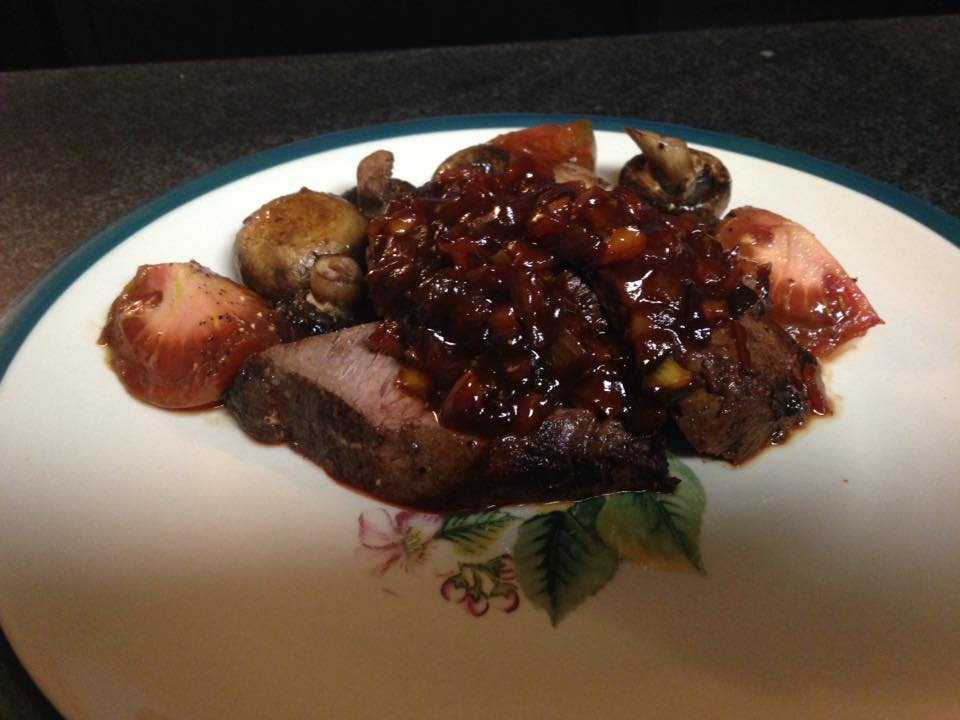
\includegraphics[height=\paperheight,%
				keepaspectratio]{./Images/VenisonBBQSauce.jpg}}%
			\vfill
}}}

%MANGOSALSA
\newcommand\MangoSalsa{%
	\put(0,0){%
		\parbox[b][\paperheight]{\paperwidth}{%
			\vfill
			\centering
			{\transparent{0.3} 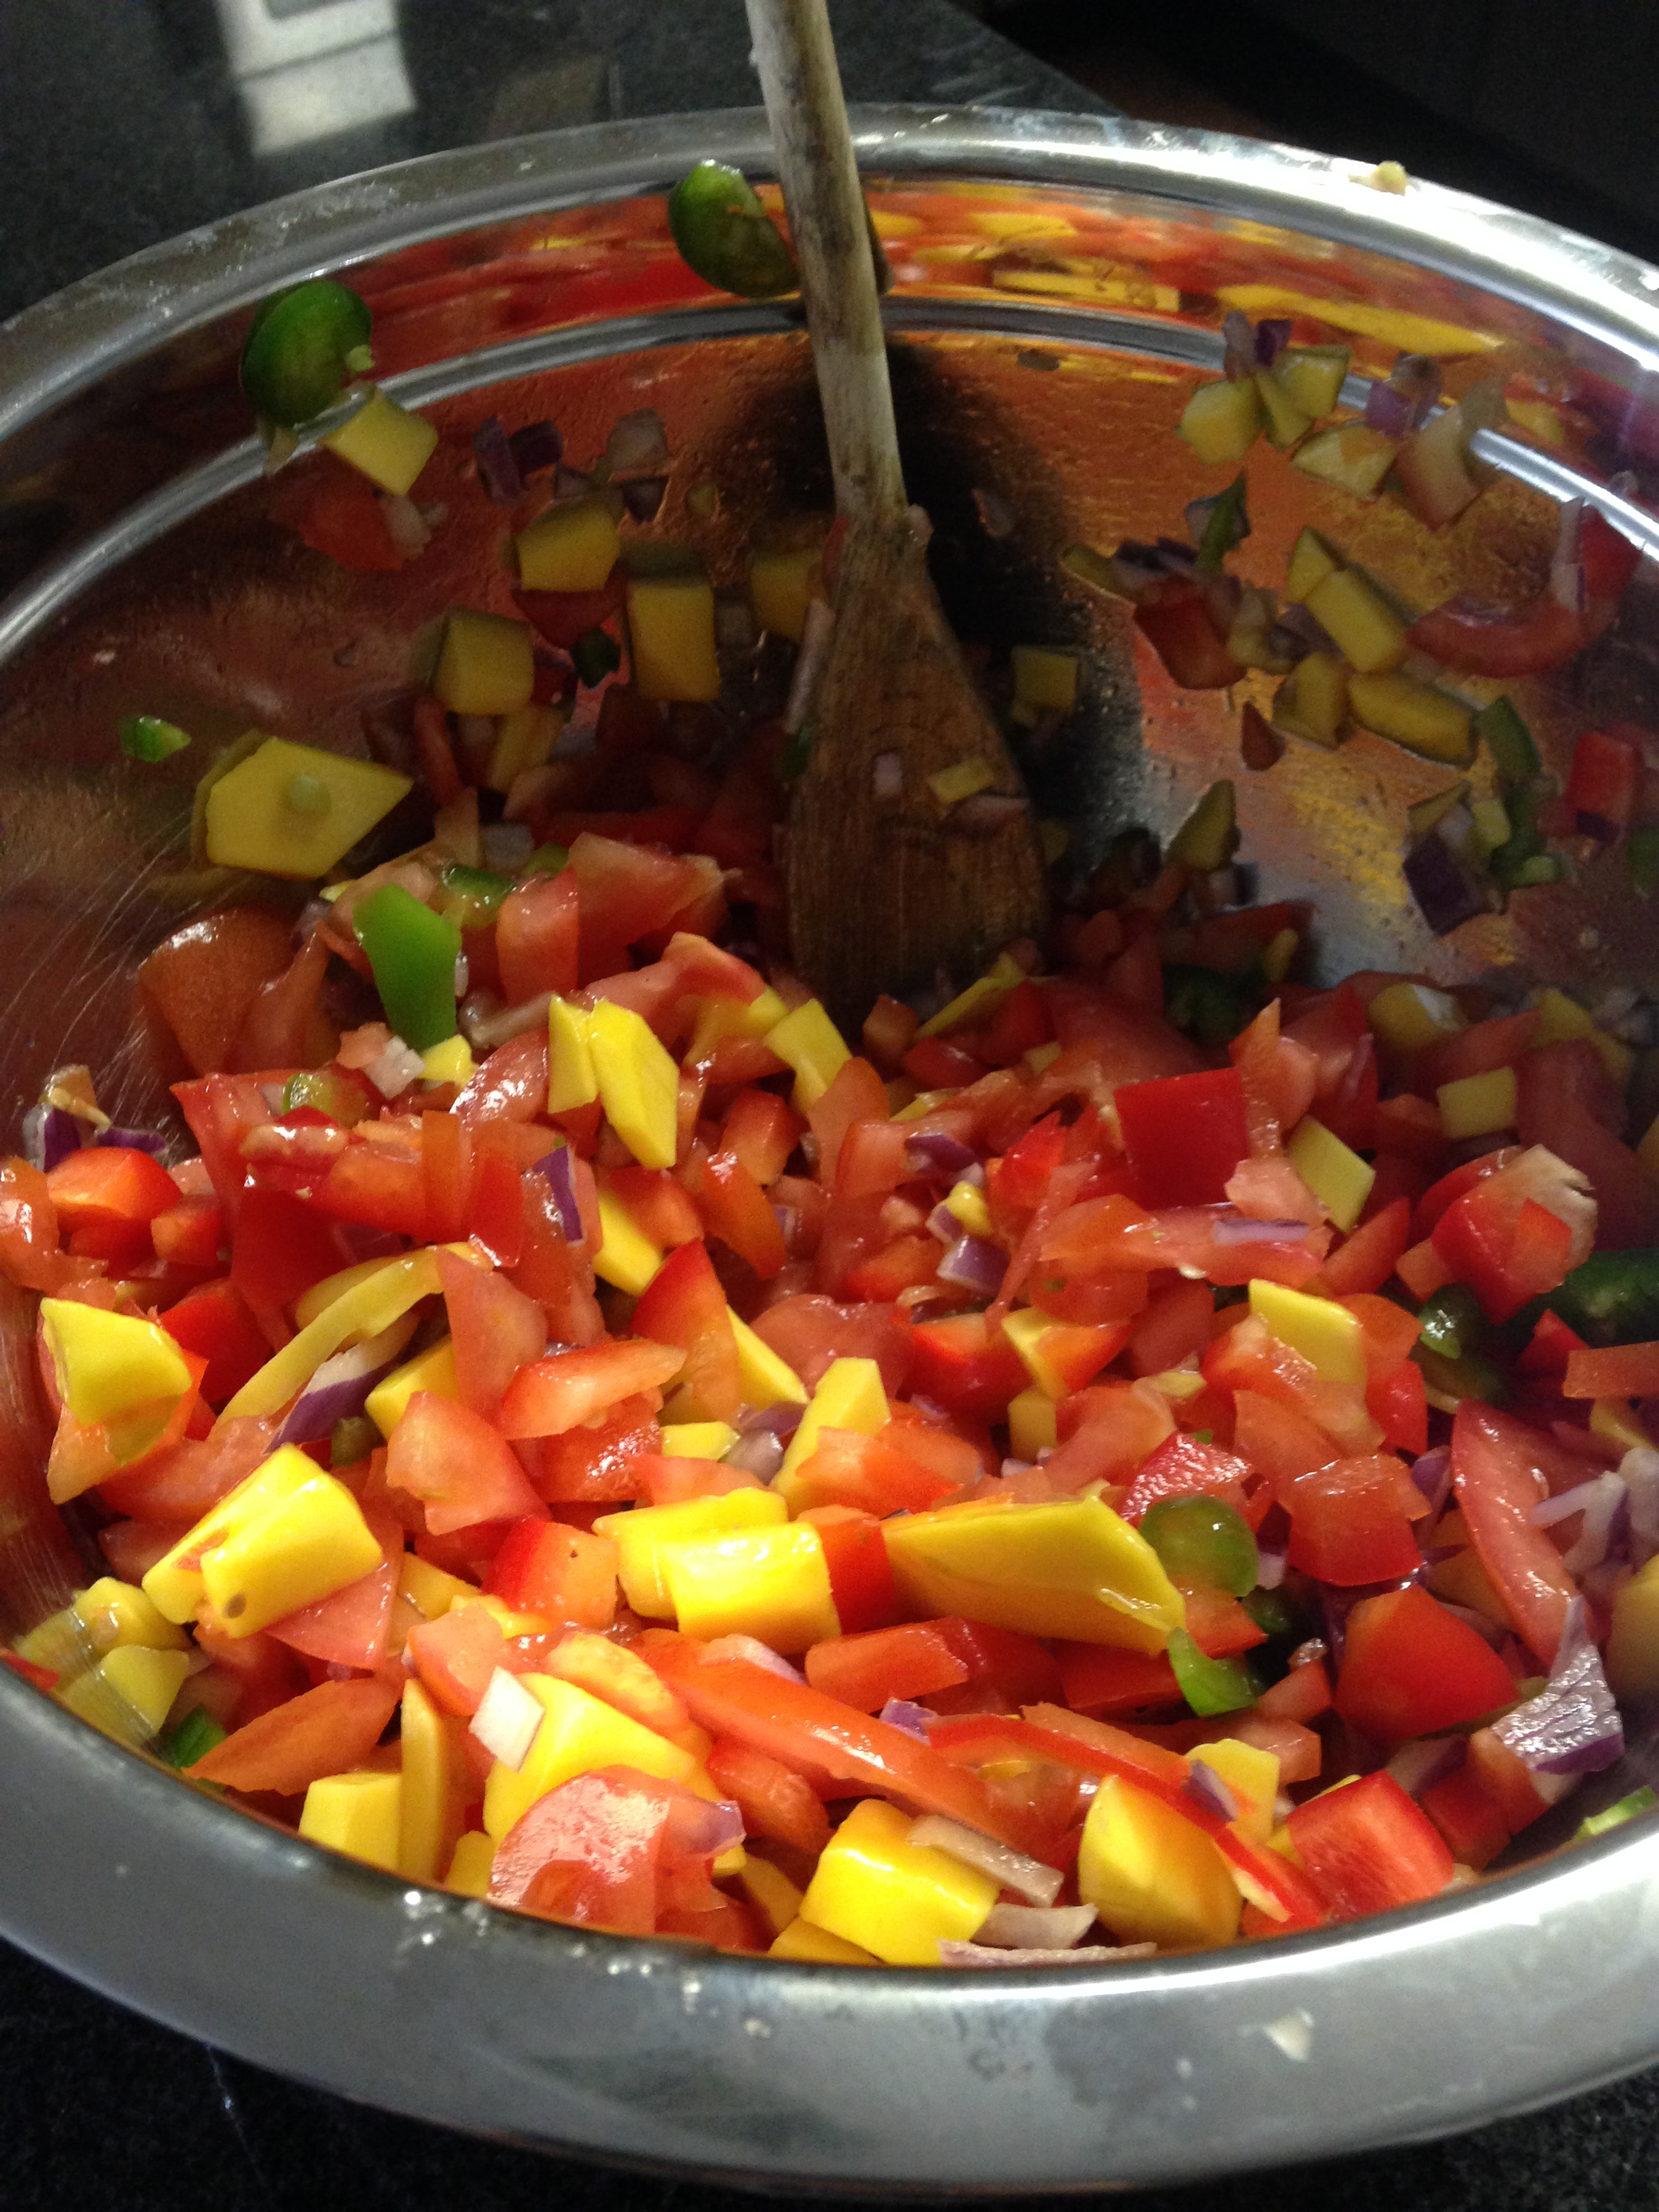
\includegraphics[height=\paperheight,%
				keepaspectratio]{./Images/MangoSalsa.jpg}}%
			\vfill
}}}

%FRUITMEDLEY
\newcommand\FruitMedley{%
	\put(0,0){%
		\parbox[b][\paperheight]{\paperwidth}{%
			\vfill
			\centering
			{\transparent{0.3} 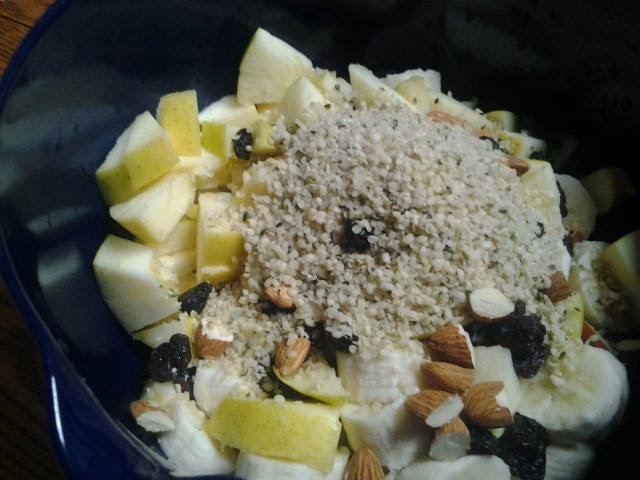
\includegraphics[height=\paperheight,%
				keepaspectratio]{./Images/FruitMedley.jpg}}%
			\vfill
}}}

%TORTILLACHIPS
\newcommand\TortillaChips{%
	\put(0,0){%
		\parbox[b][\paperheight]{\paperwidth}{%
			\vfill
			\centering
			{\transparent{0.3} 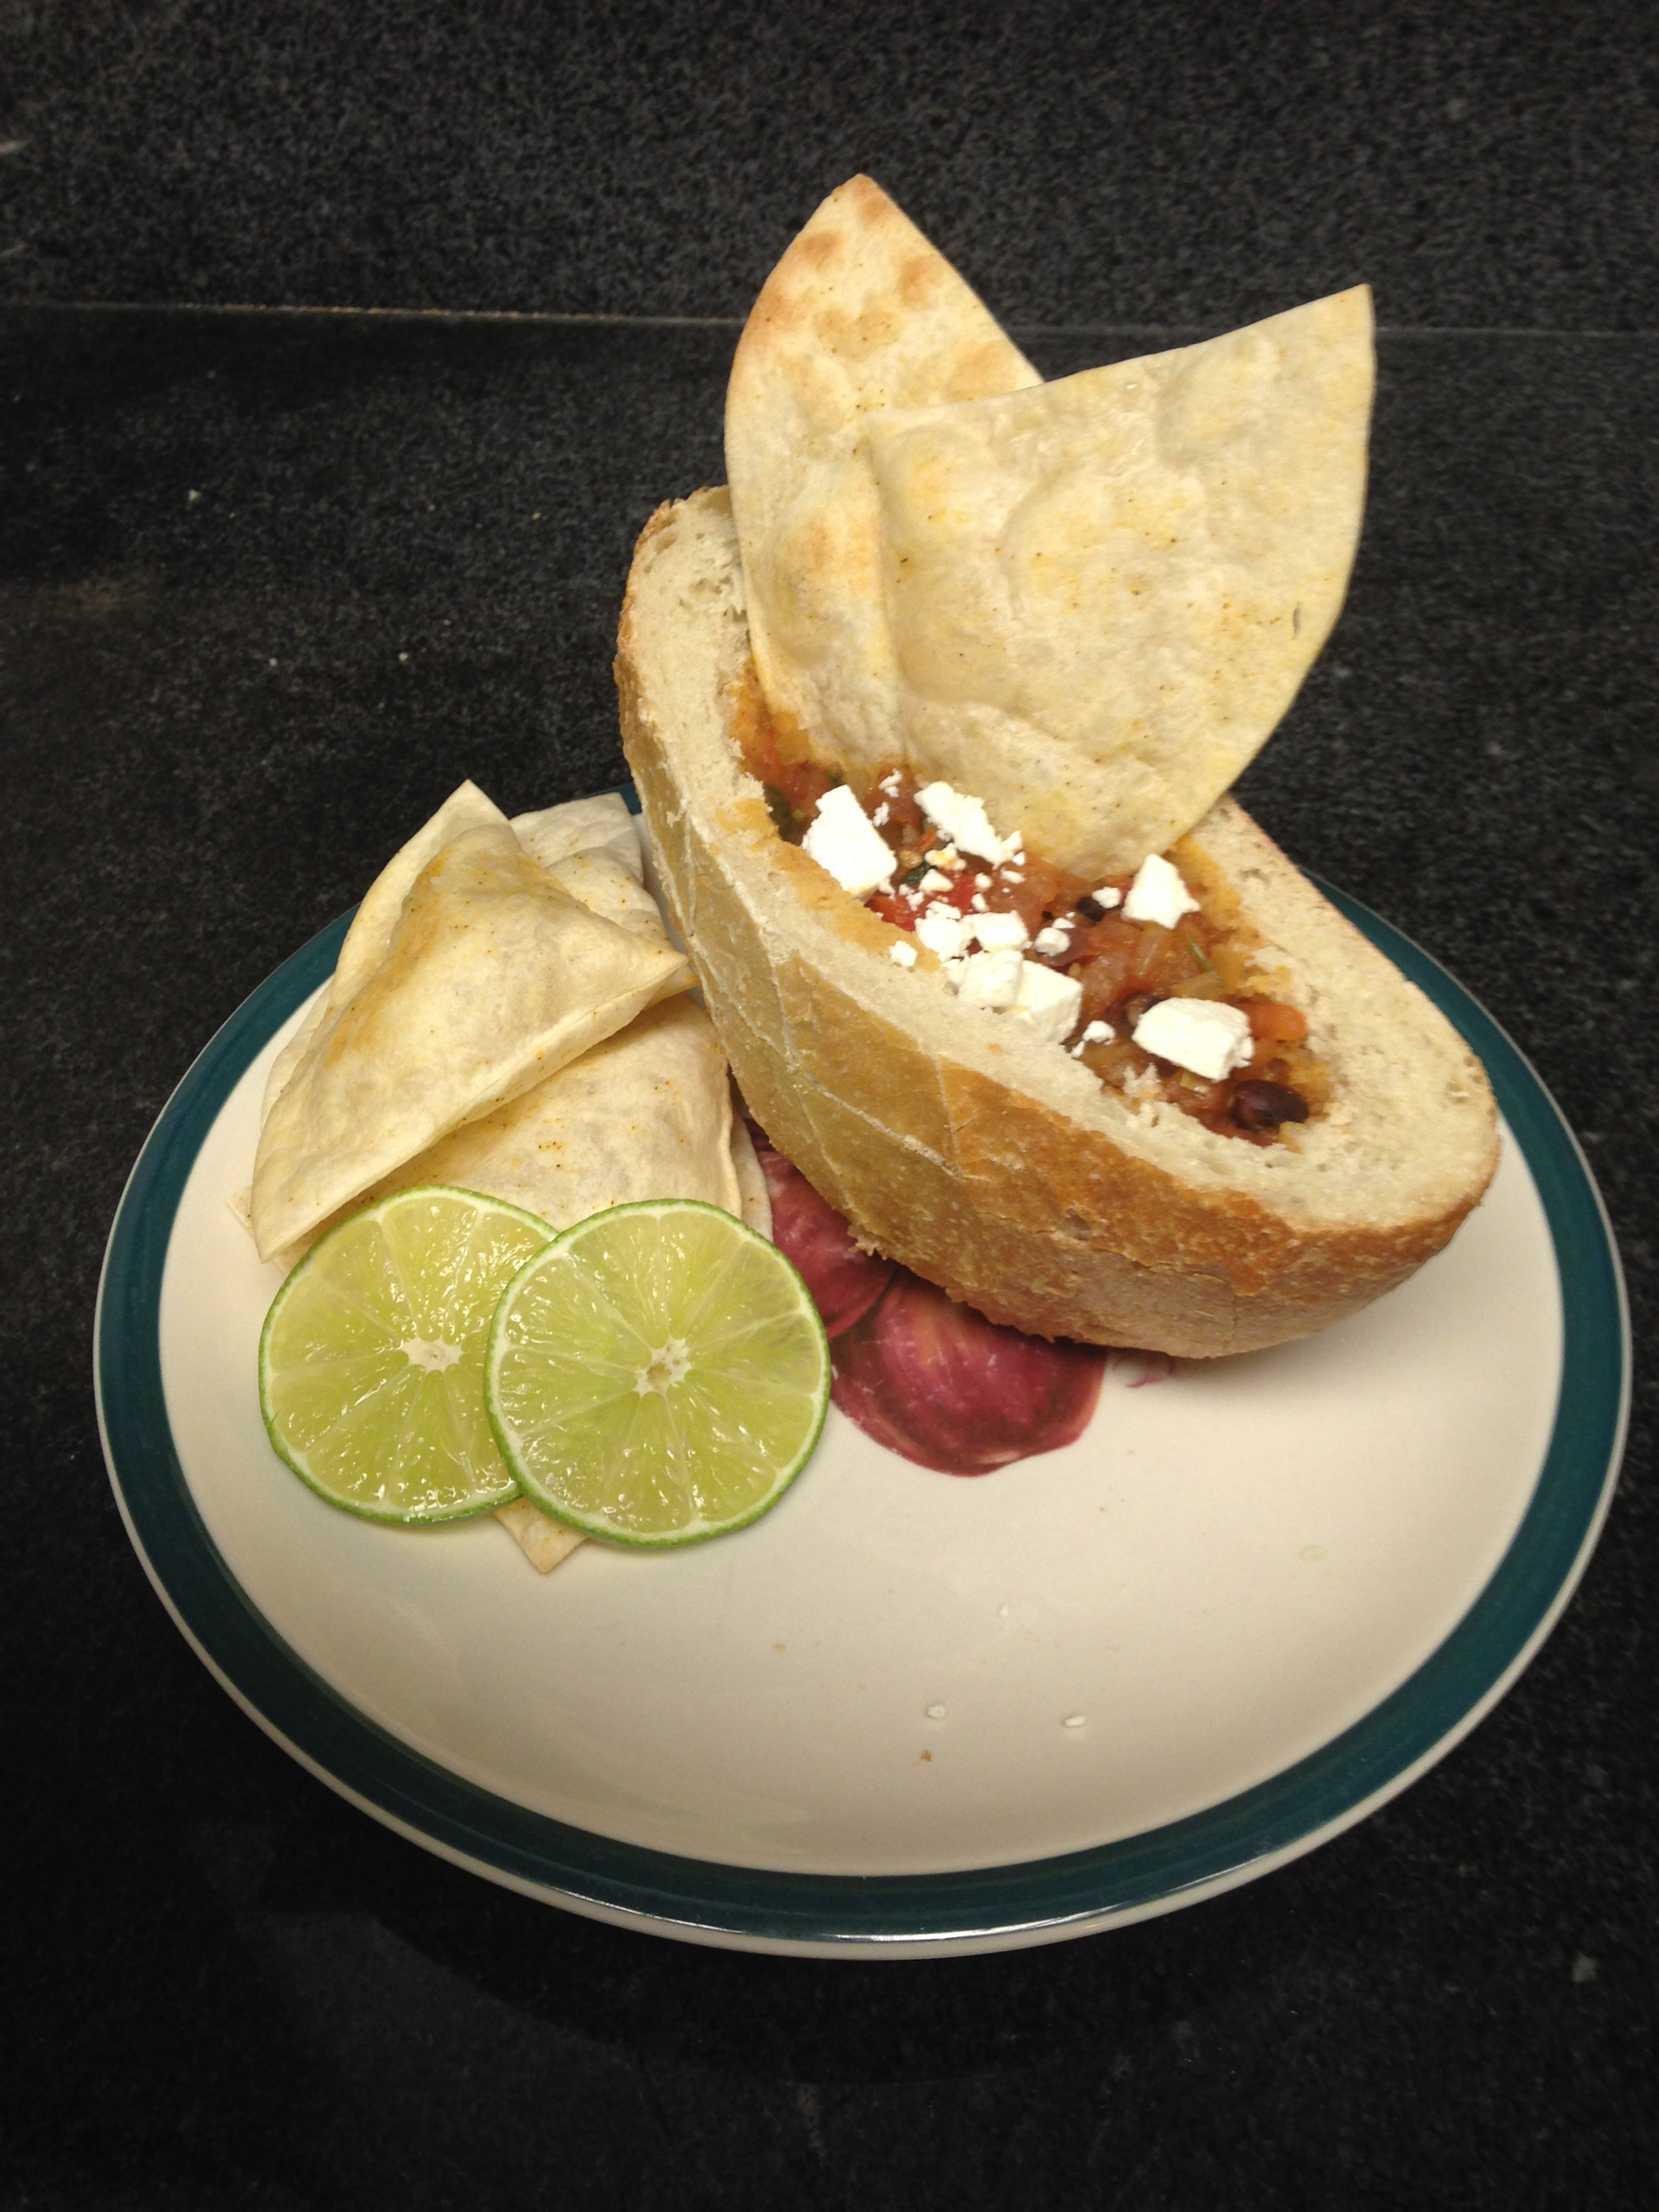
\includegraphics[height=\paperheight,%
				keepaspectratio]{./Images/TortillaChips.jpg}}%
			\vfill
}}}

%FRUITTOPPING
\newcommand\FruitTopping{%
	\put(0,0){%
		\parbox[b][\paperheight]{\paperwidth}{%
			\vfill
			\centering
			{\transparent{0.3} 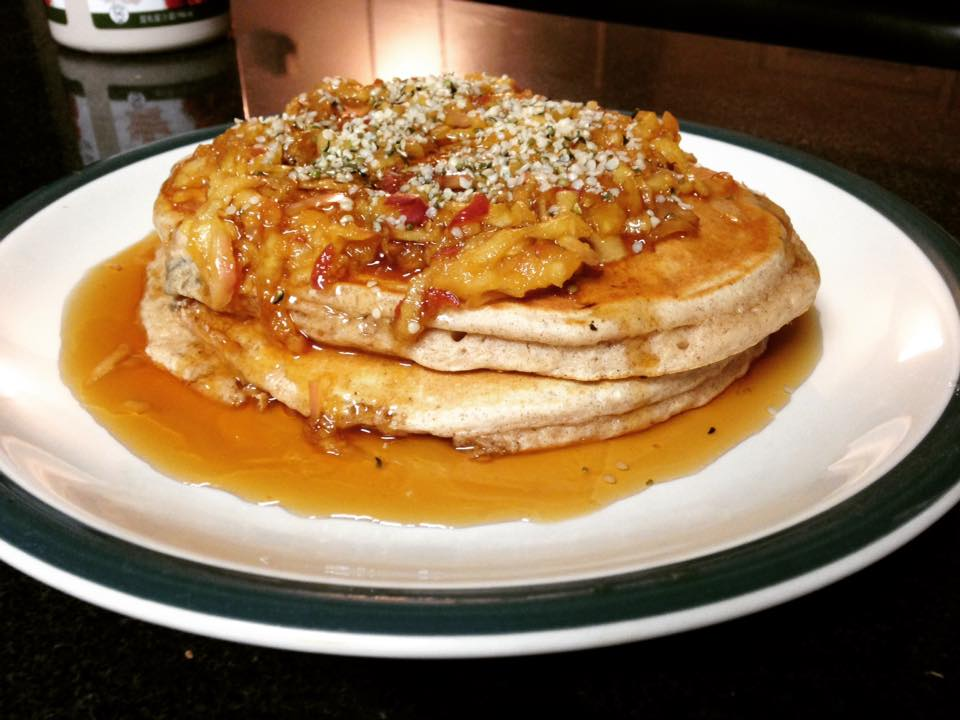
\includegraphics[height=\paperheight,%
				keepaspectratio]{./Images/PancakesWithApple.jpg}}%
			\vfill
}}}

%LEMONPOPPYSEED
\newcommand\LemonPoppyseed{%
	\put(0,0){%
		\parbox[b][\paperheight]{\paperwidth}{%
			\vfill
			\centering
			{\transparent{0.3} 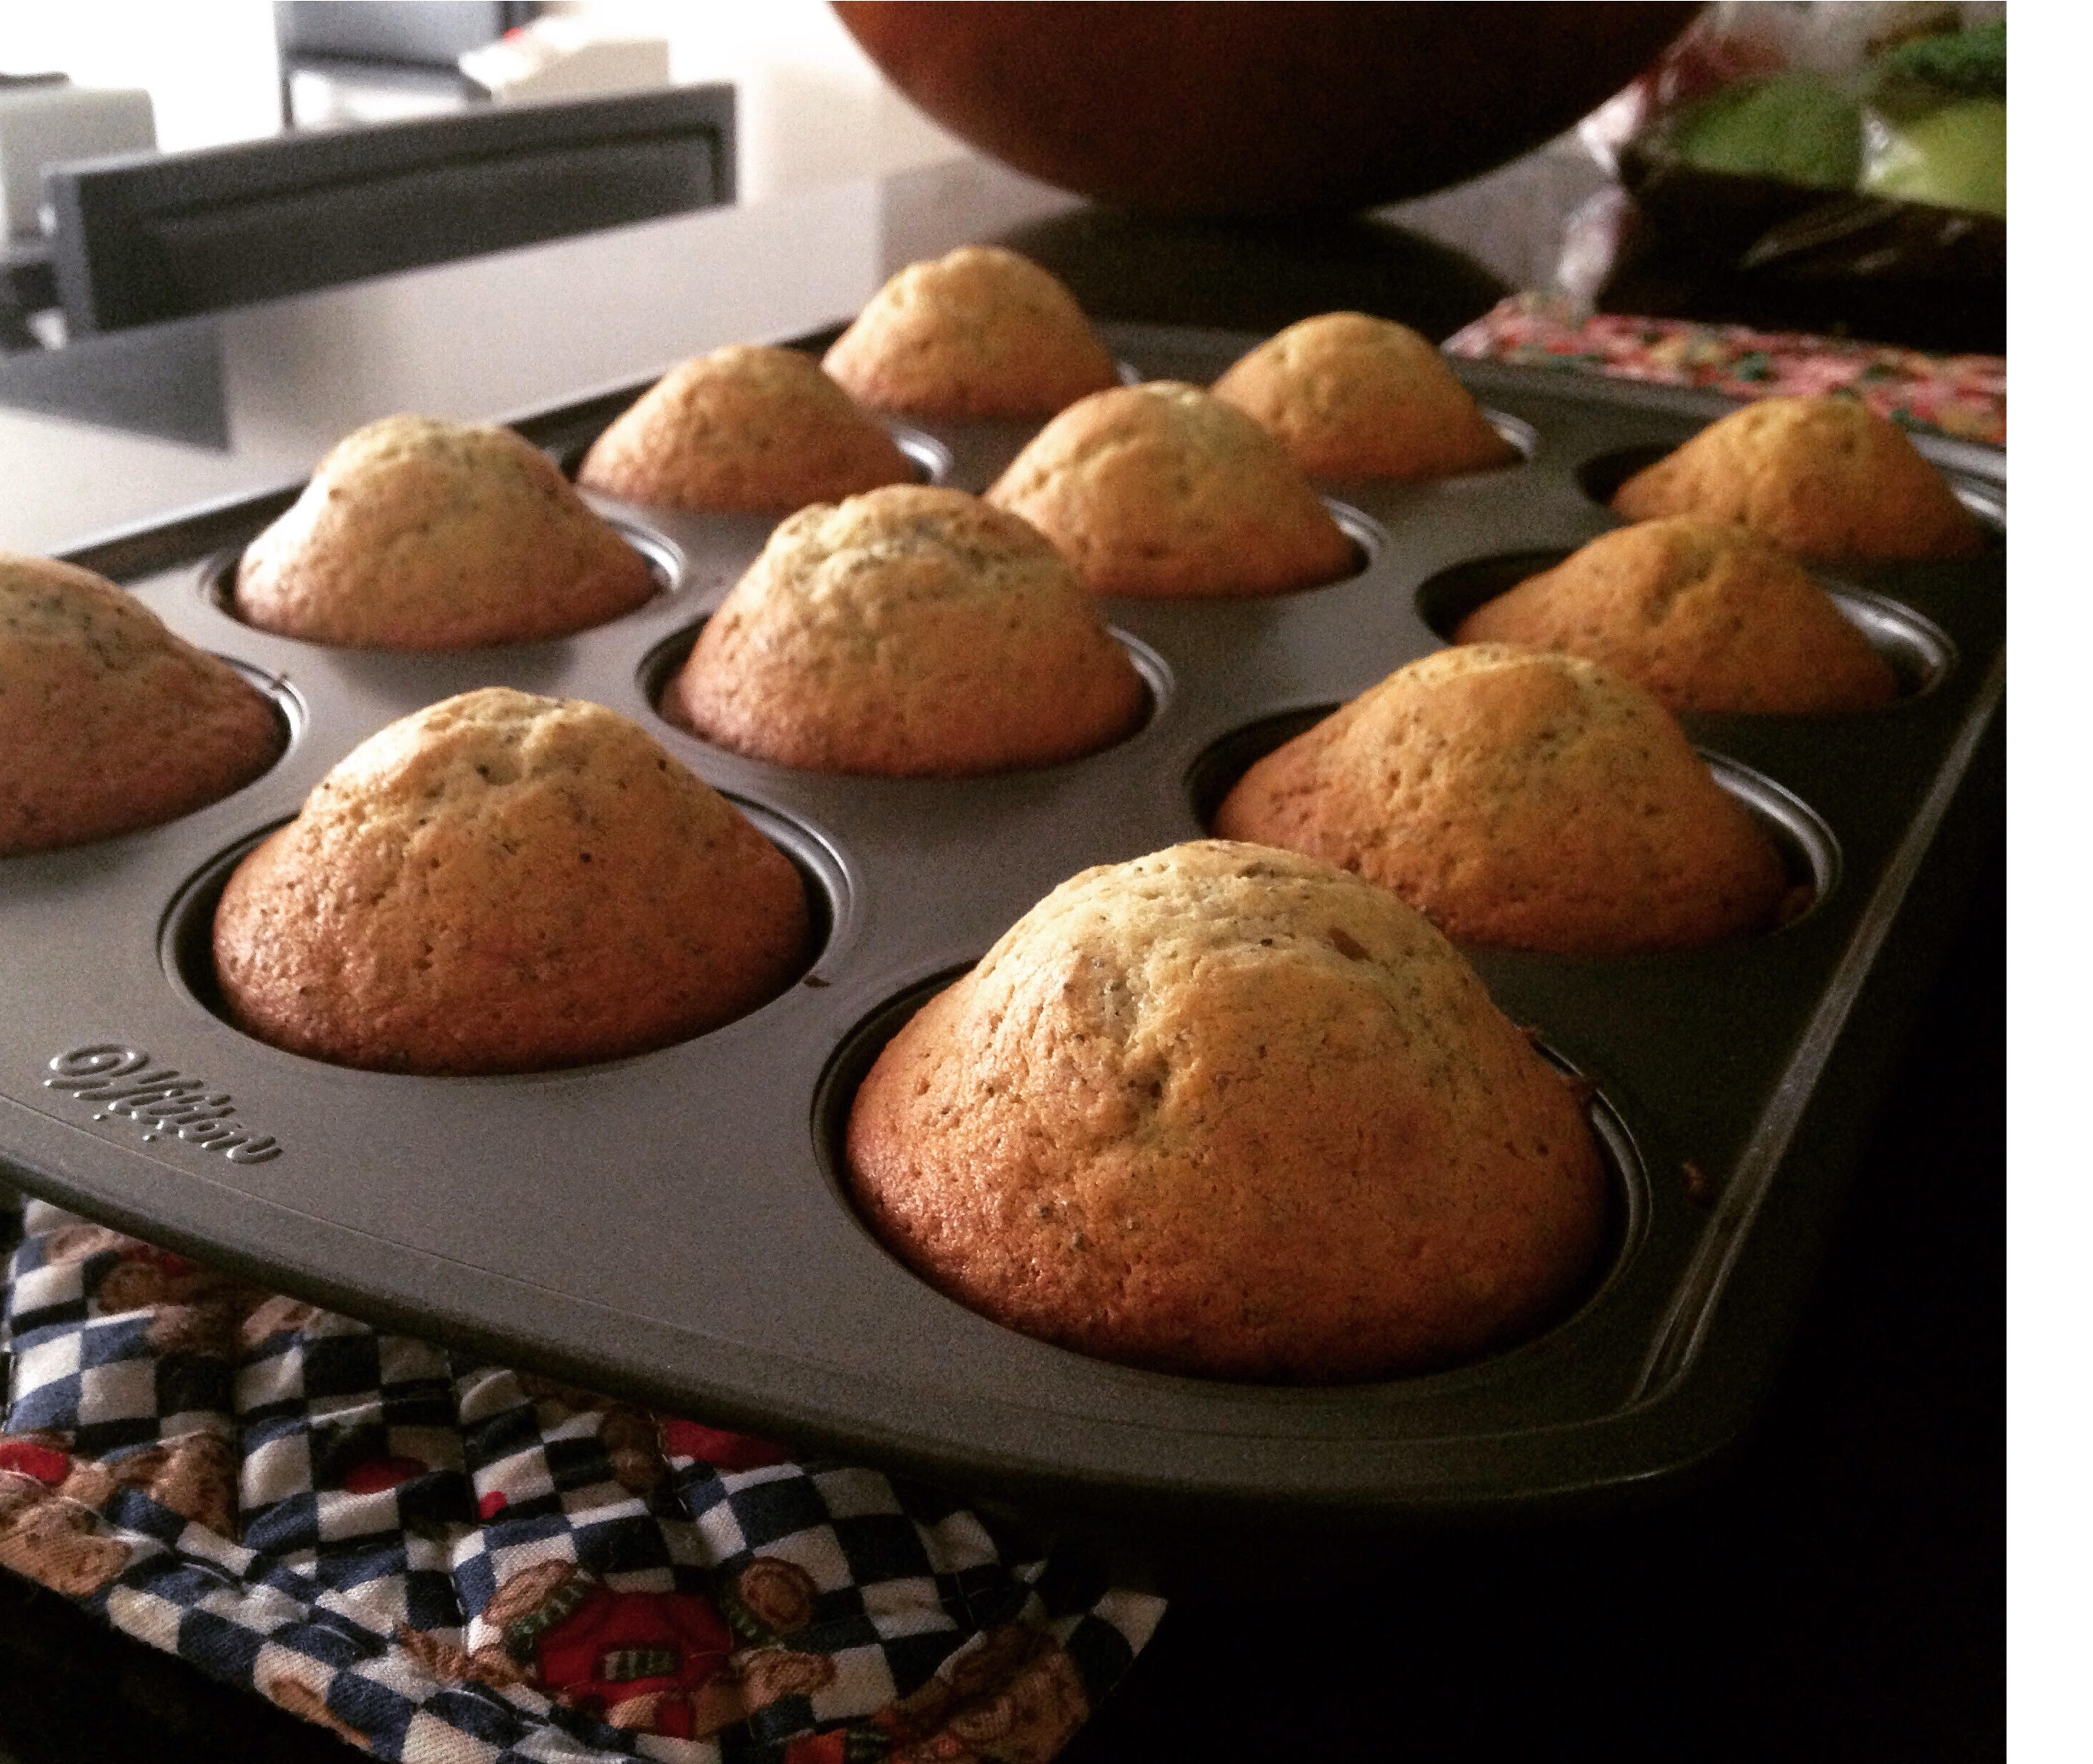
\includegraphics[height=\paperheight,%
				keepaspectratio]{./Images/LemonPoppyseed.jpg}}%
			\vfill
}}}

%TOWERGARDEN
\newcommand\TowerGarden{%
	\put(0,0){%
		\parbox[b][\paperheight]{\paperwidth}{%
			\vfill
			\centering
			{\transparent{0.3} 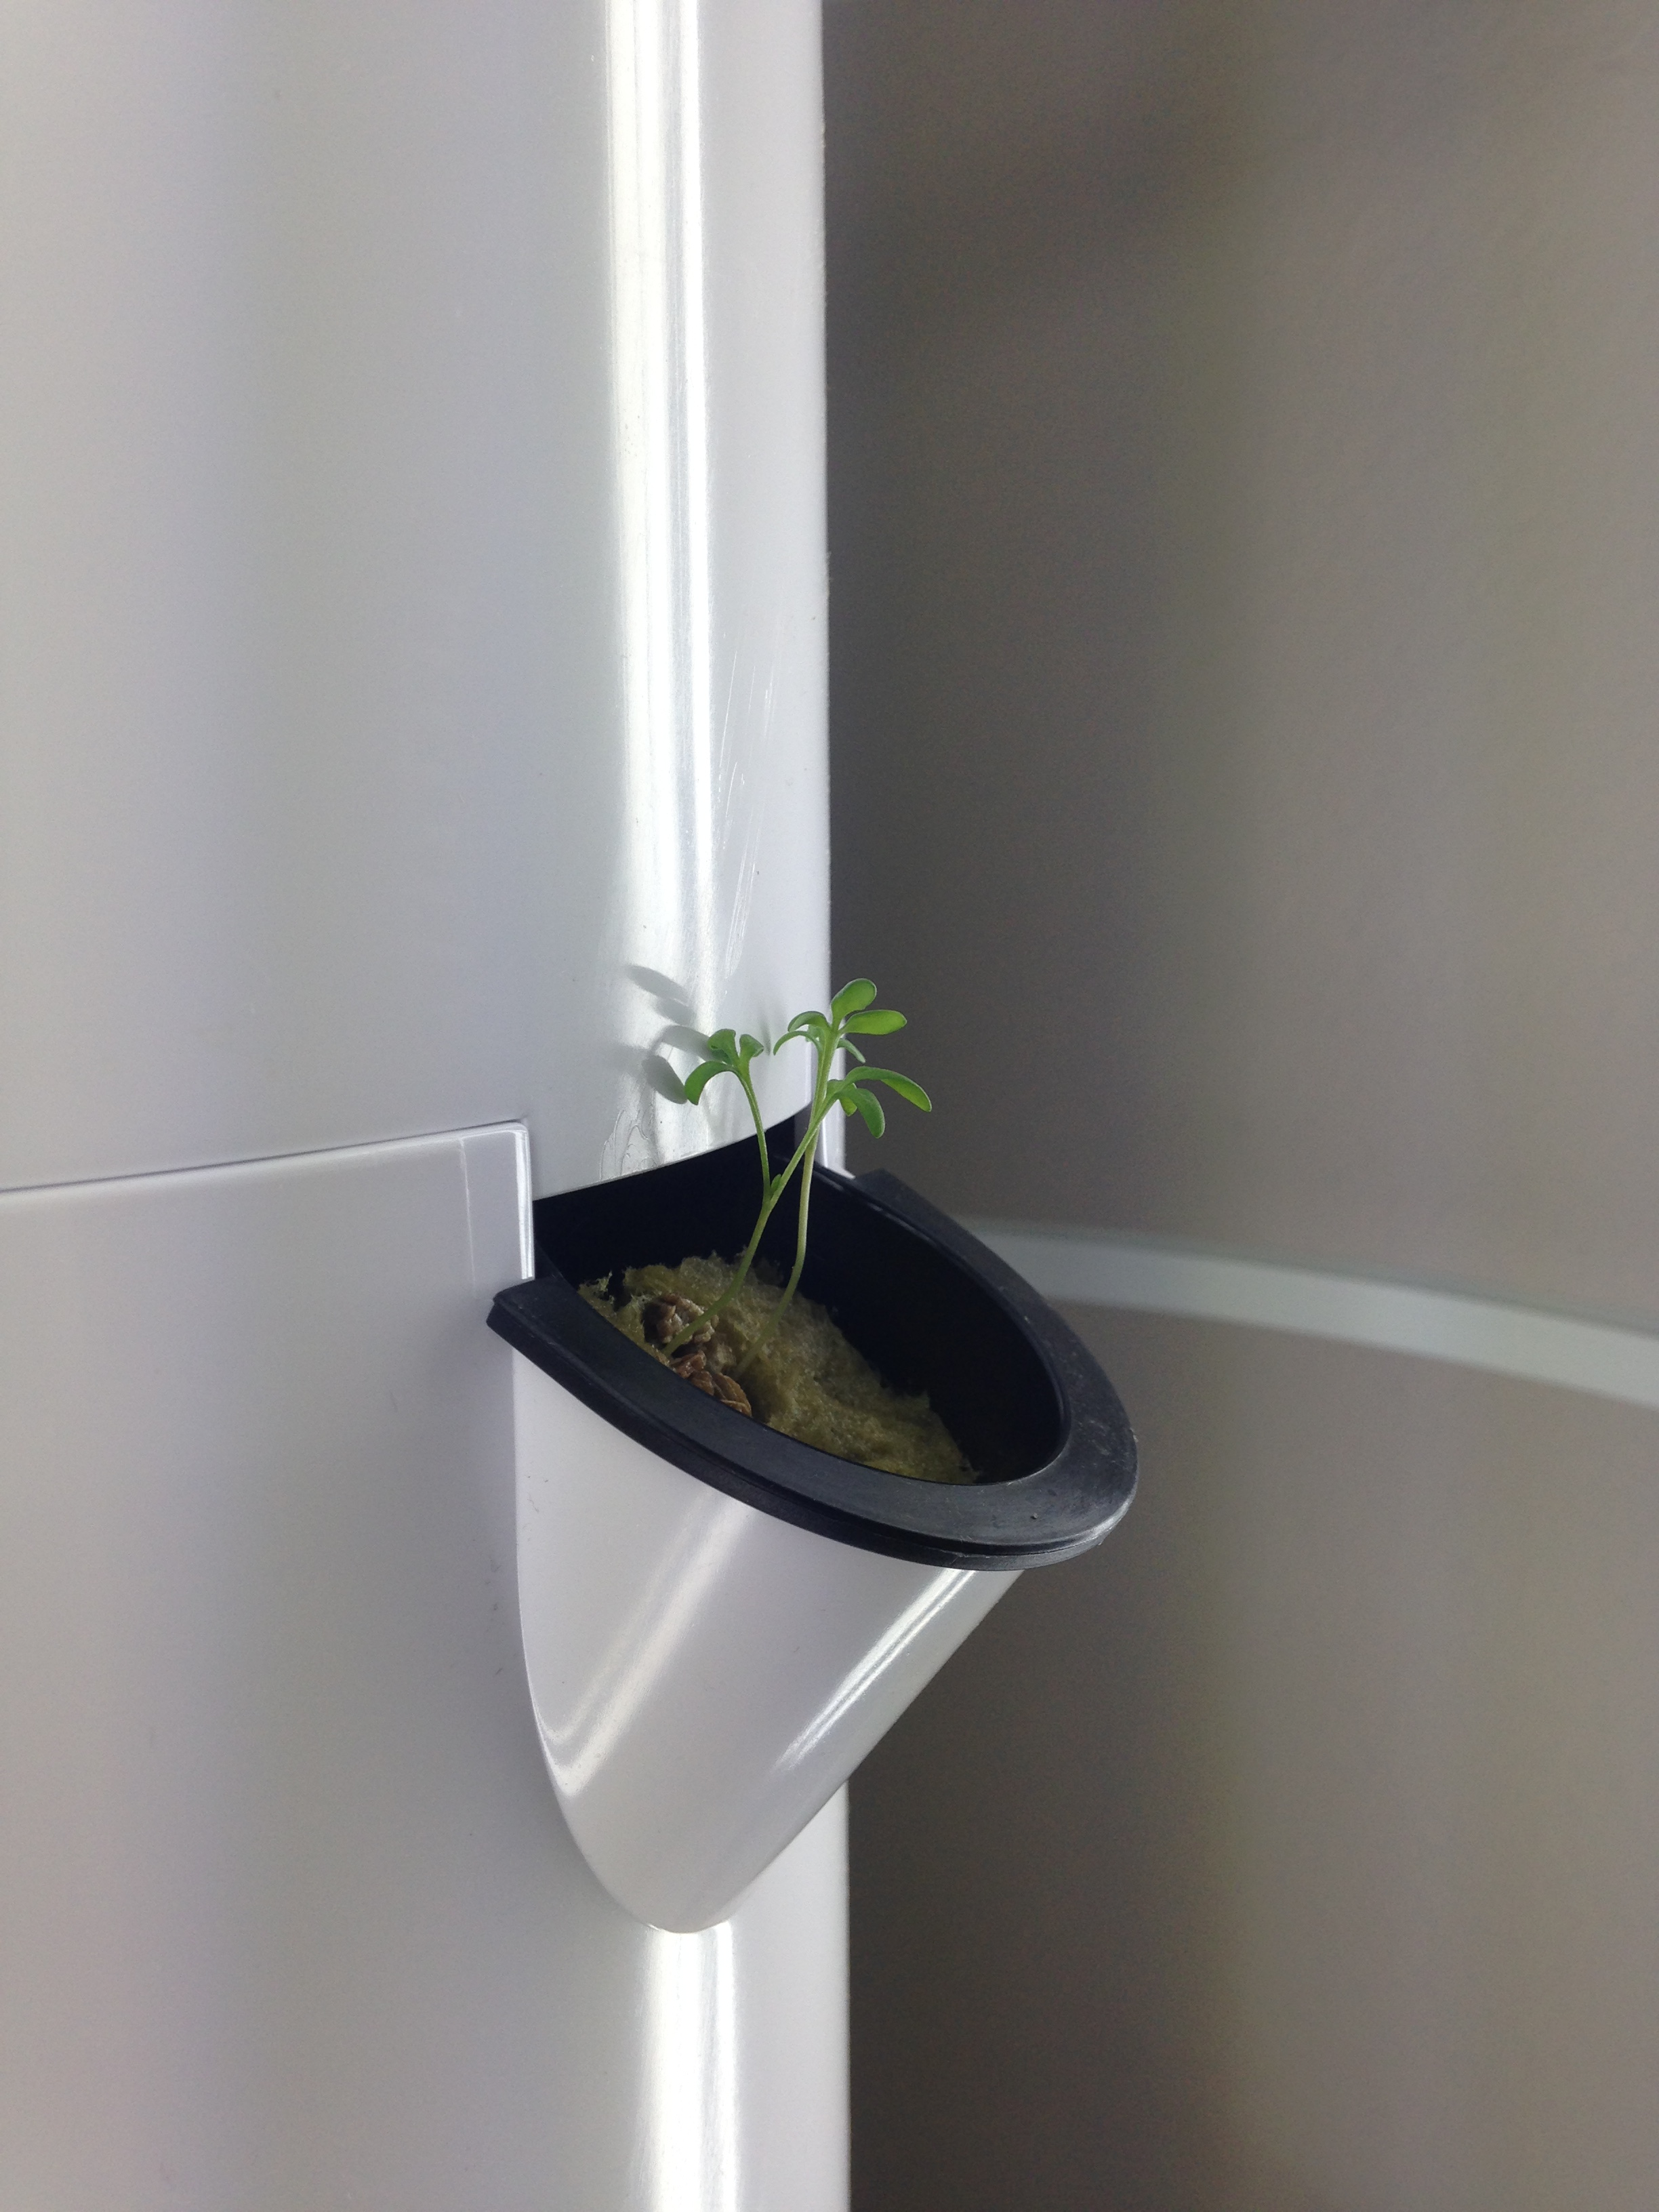
\includegraphics[height=\paperheight,%
				keepaspectratio]{./Images/TowerGarden.jpg}}%
			\vfill
}}}

%SAFFRONICECREAM
\newcommand\SaffronIceCream{%
	\put(0,0){%
		\parbox[b][\paperheight]{\paperwidth}{%
			\vfill
			\centering
			{\transparent{0.3} 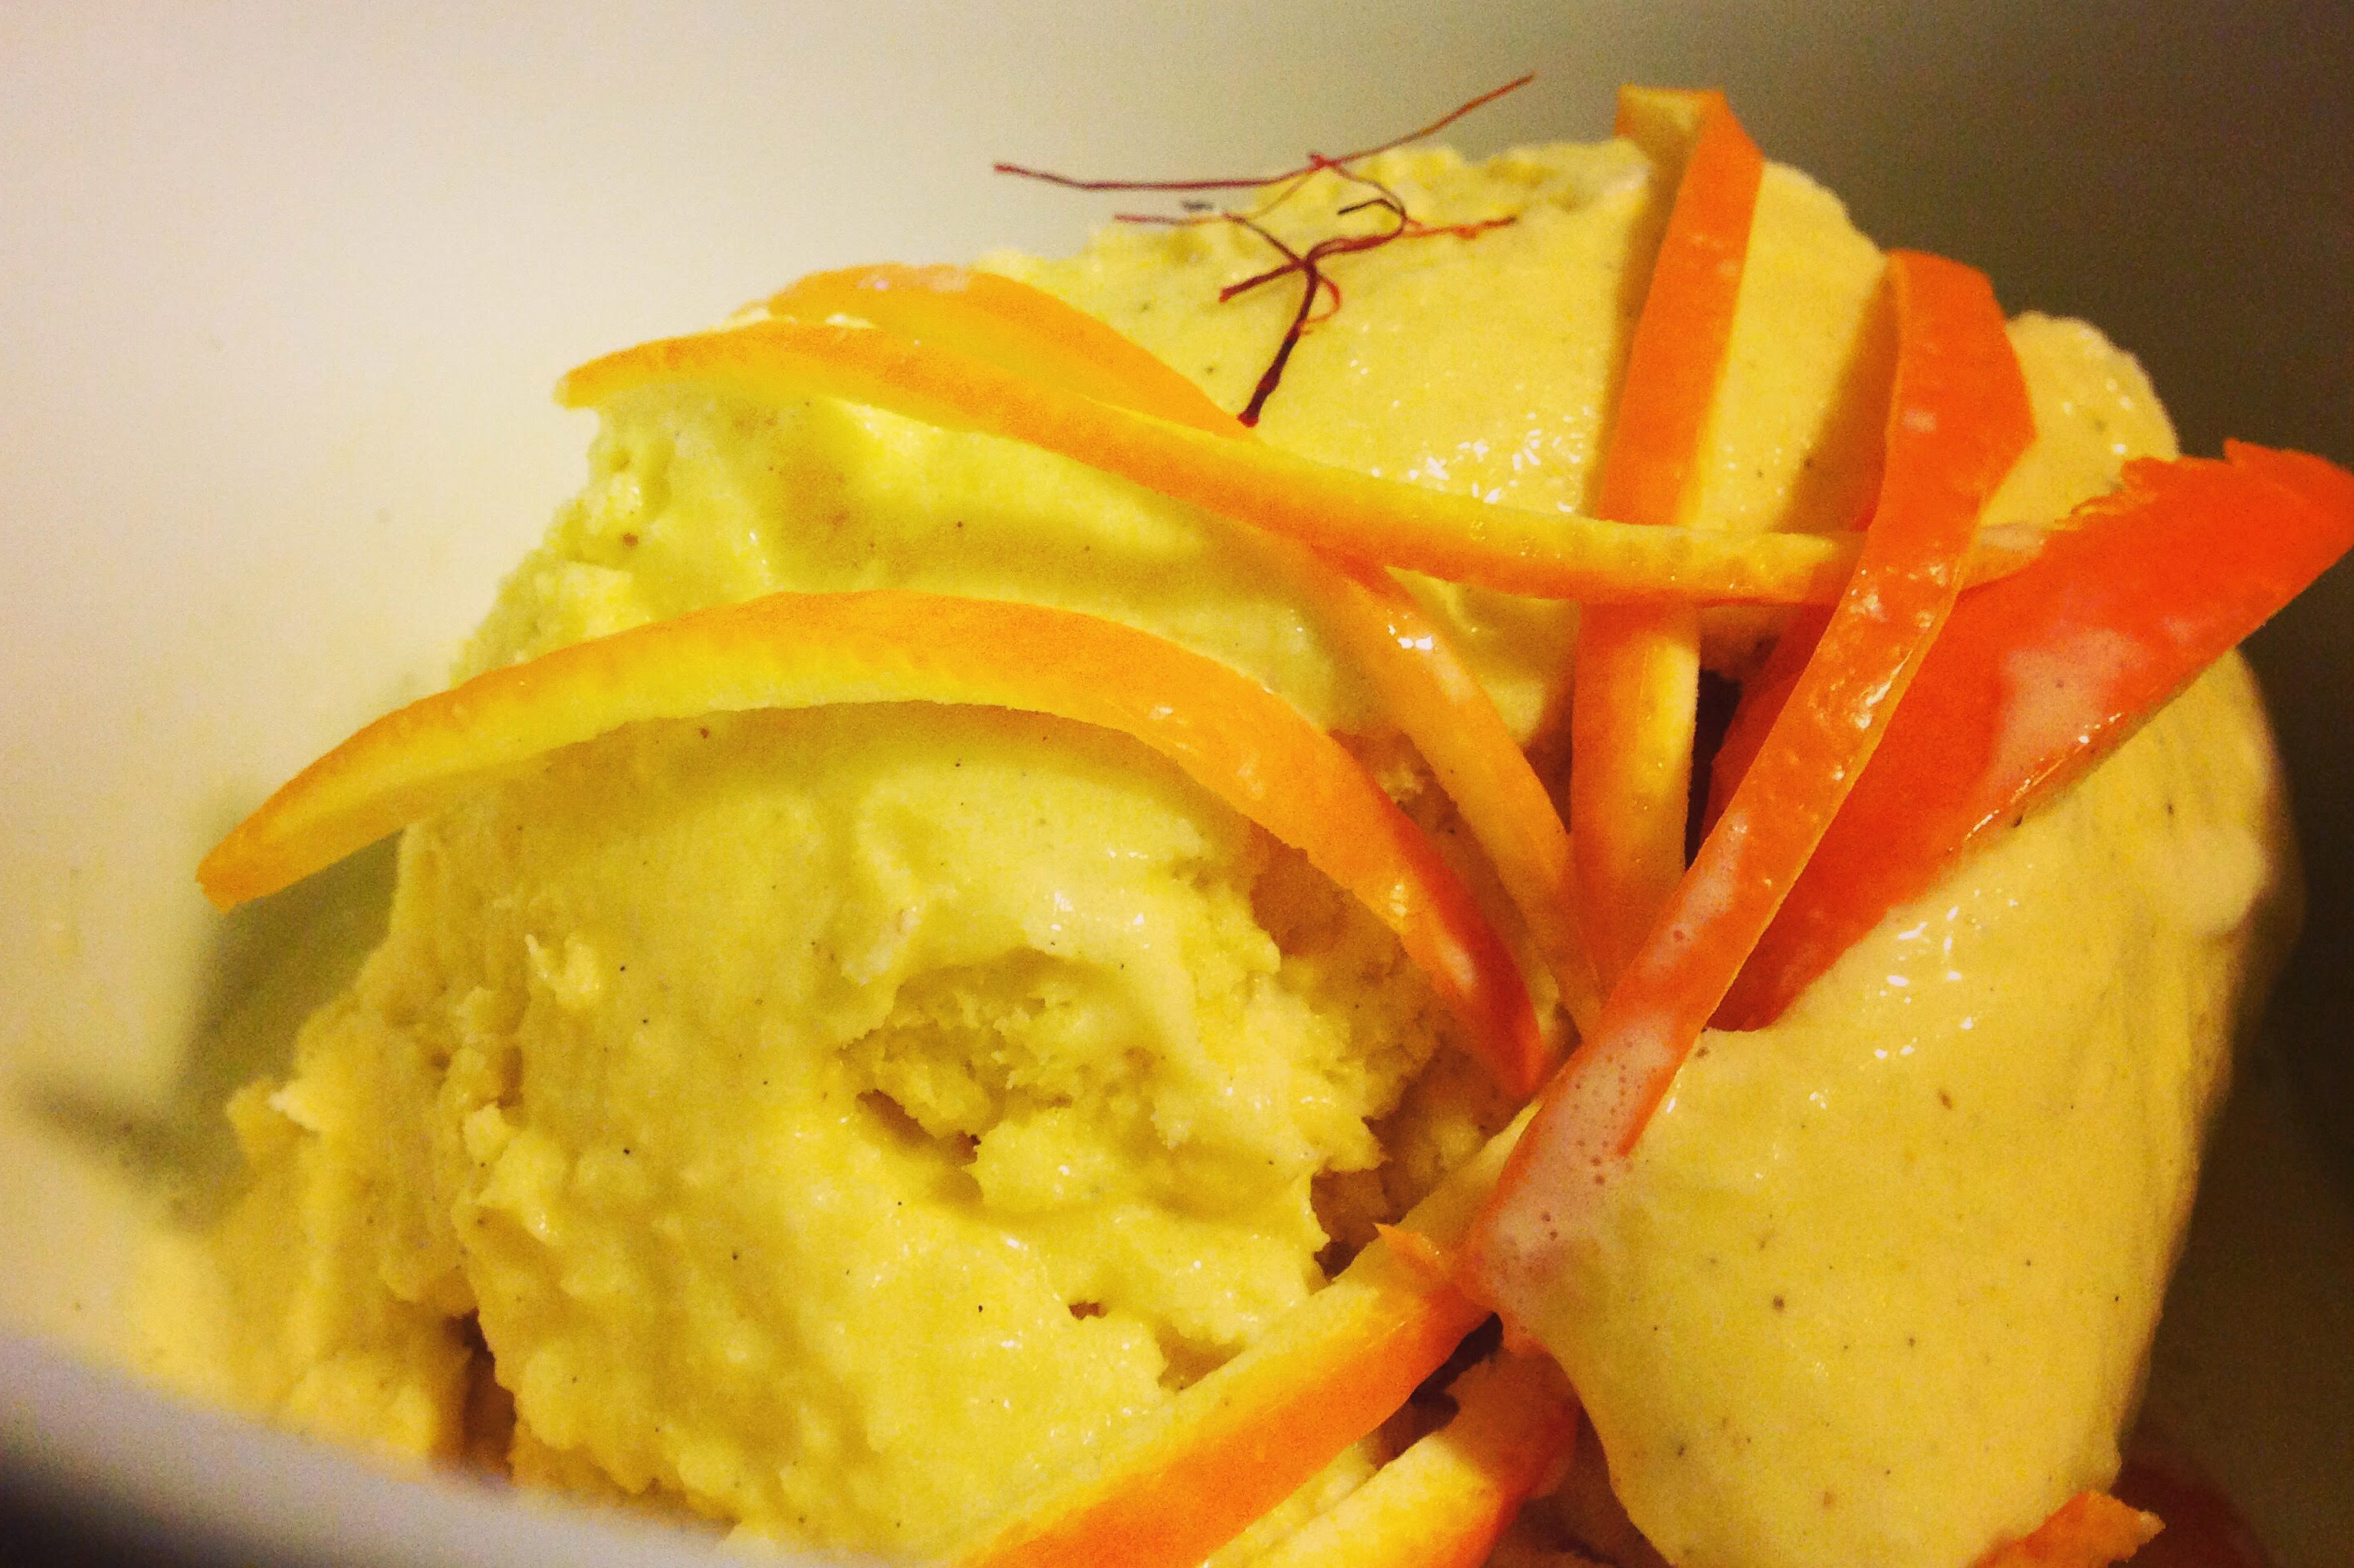
\includegraphics[height=\paperheight,%
				keepaspectratio]{./Images/SaffronIceCream.jpg}}%
			\vfill
}}}

%STRAWBERRYSALAD
\newcommand\StrawberrySalad{%


	\put(0,0){%
		\parbox[b][\paperheight]{\paperwidth}{%
			\vfill
			\centering
			{\transparent{0.3} 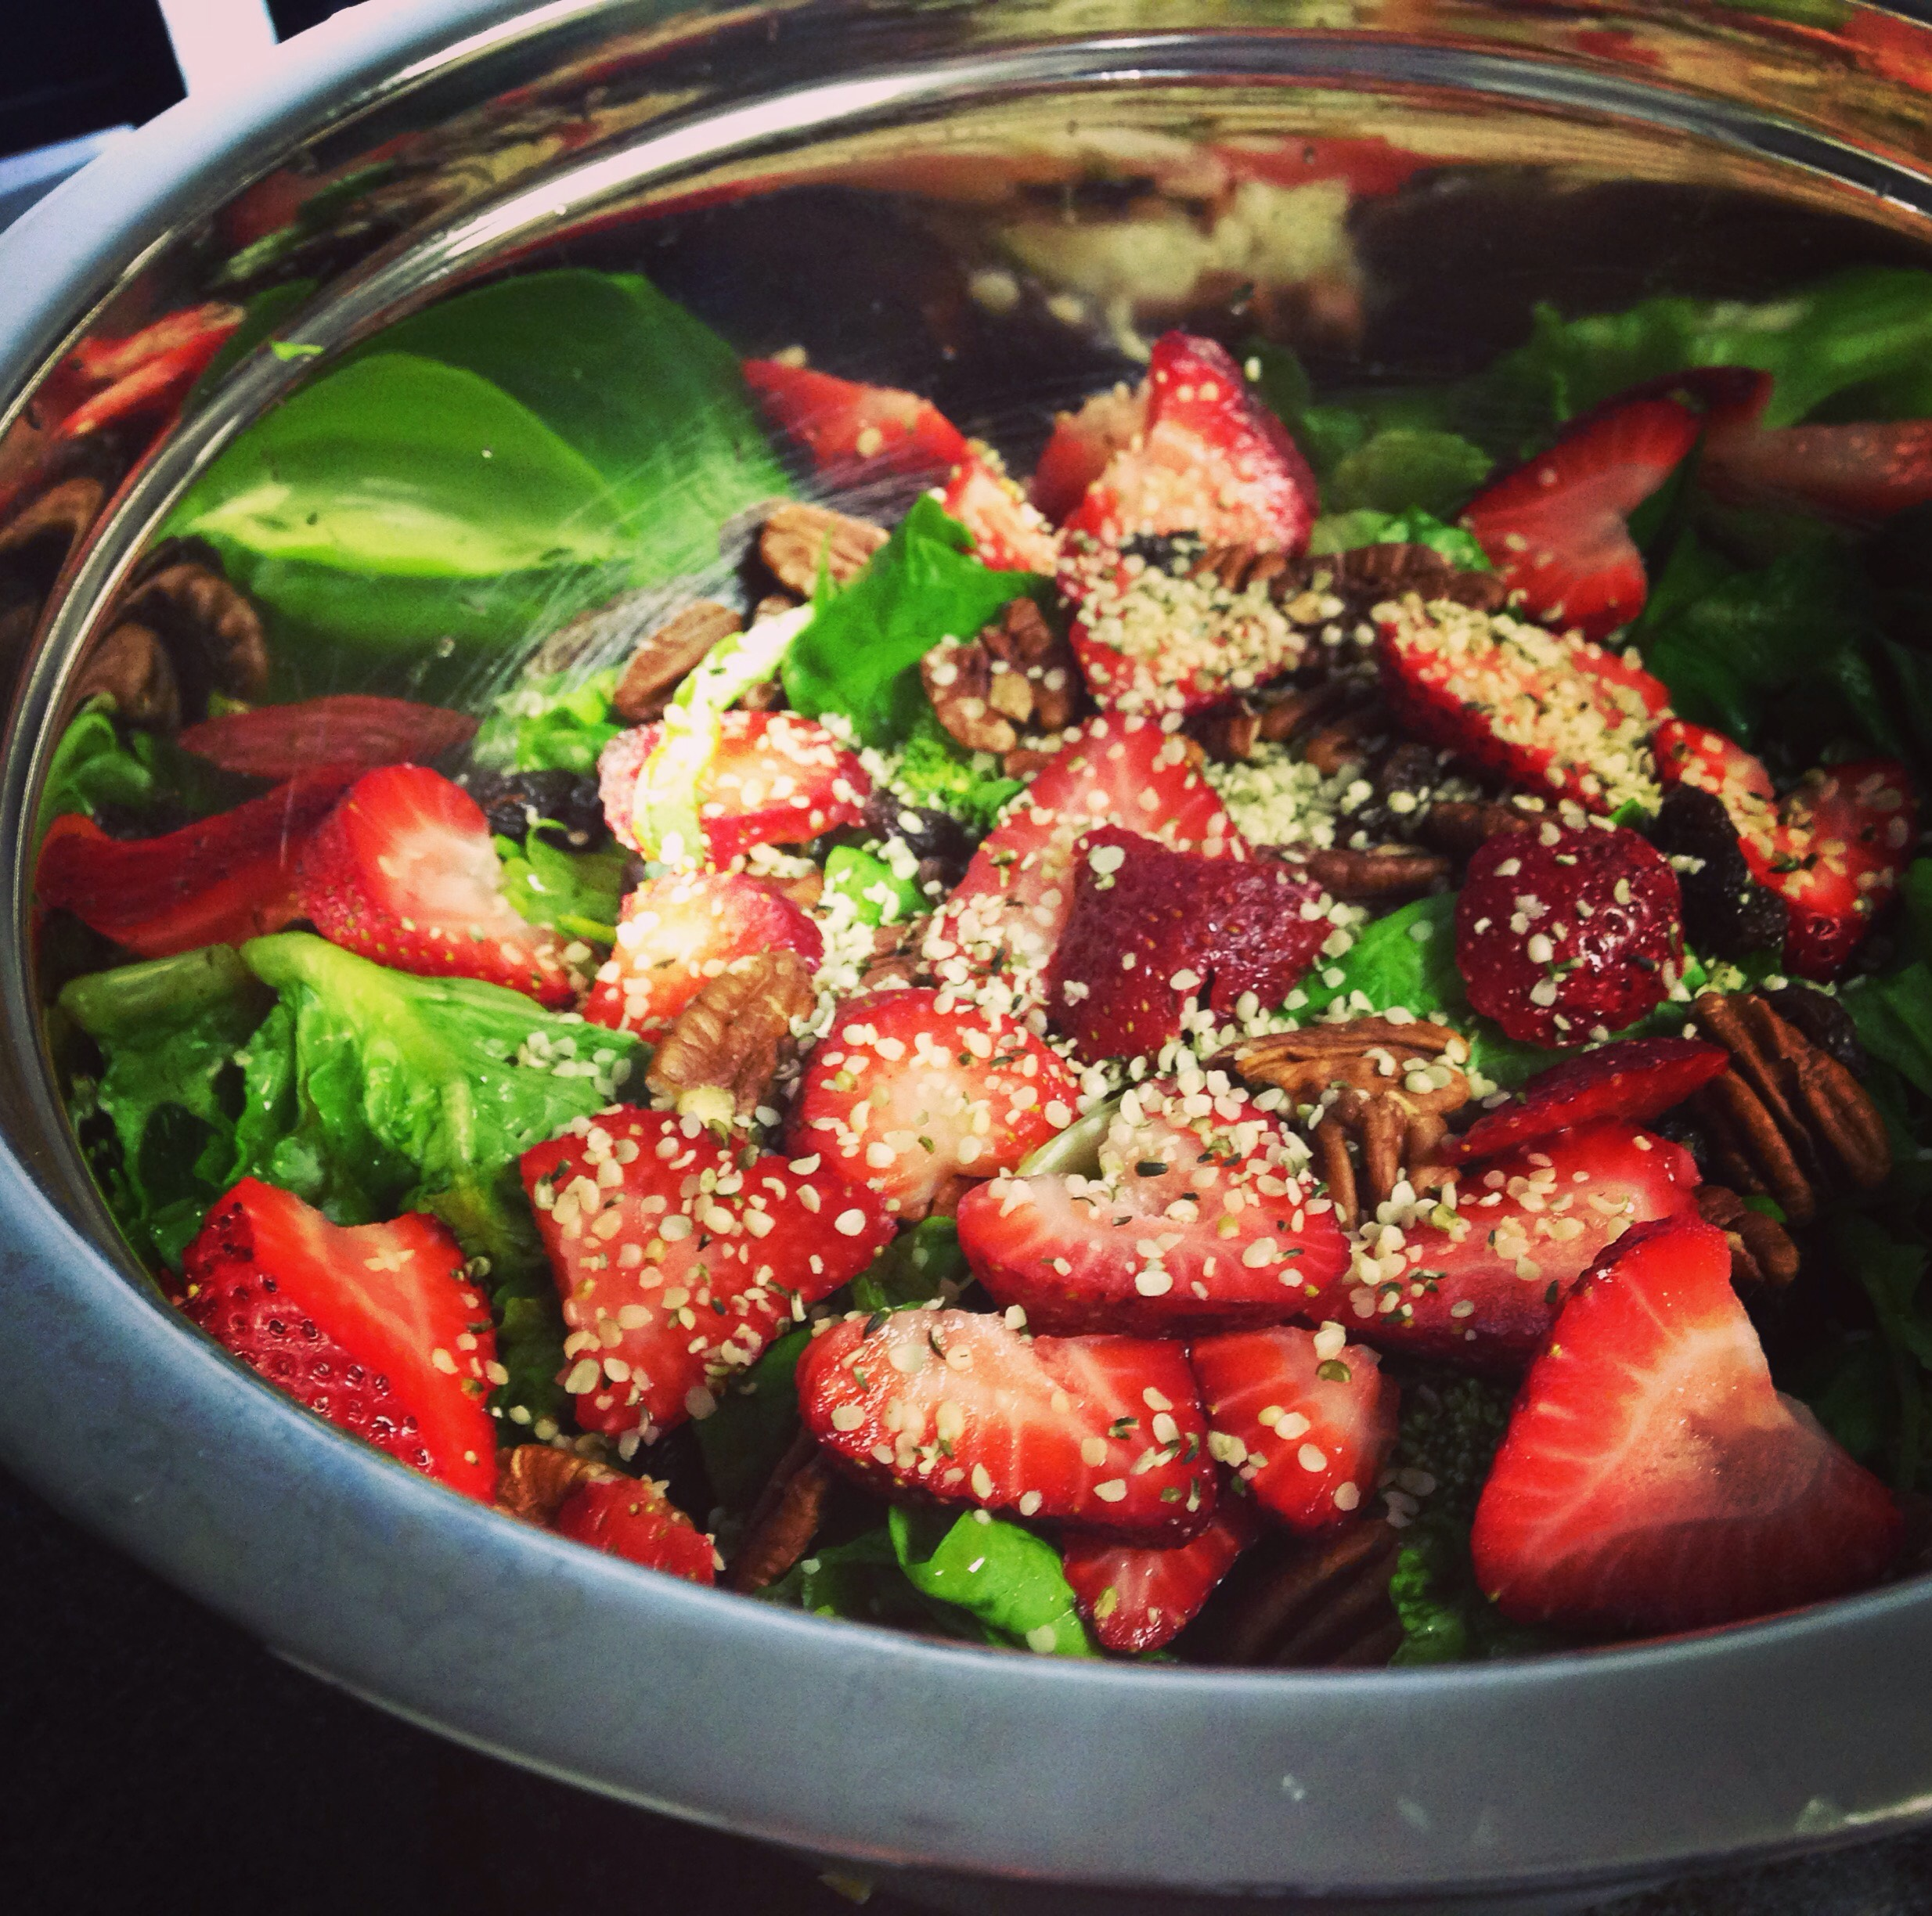
\includegraphics[height=\paperheight,%
				keepaspectratio]{./Images/StrawberrySalad.jpg}}%
			\vfill
}}}

%SALMONSALAD
\newcommand\SalmonSalad{%
	
	
	\put(0,0){%
		\parbox[b][\paperheight]{\paperwidth}{%
			\vfill
			\centering
			{\transparent{0.3} 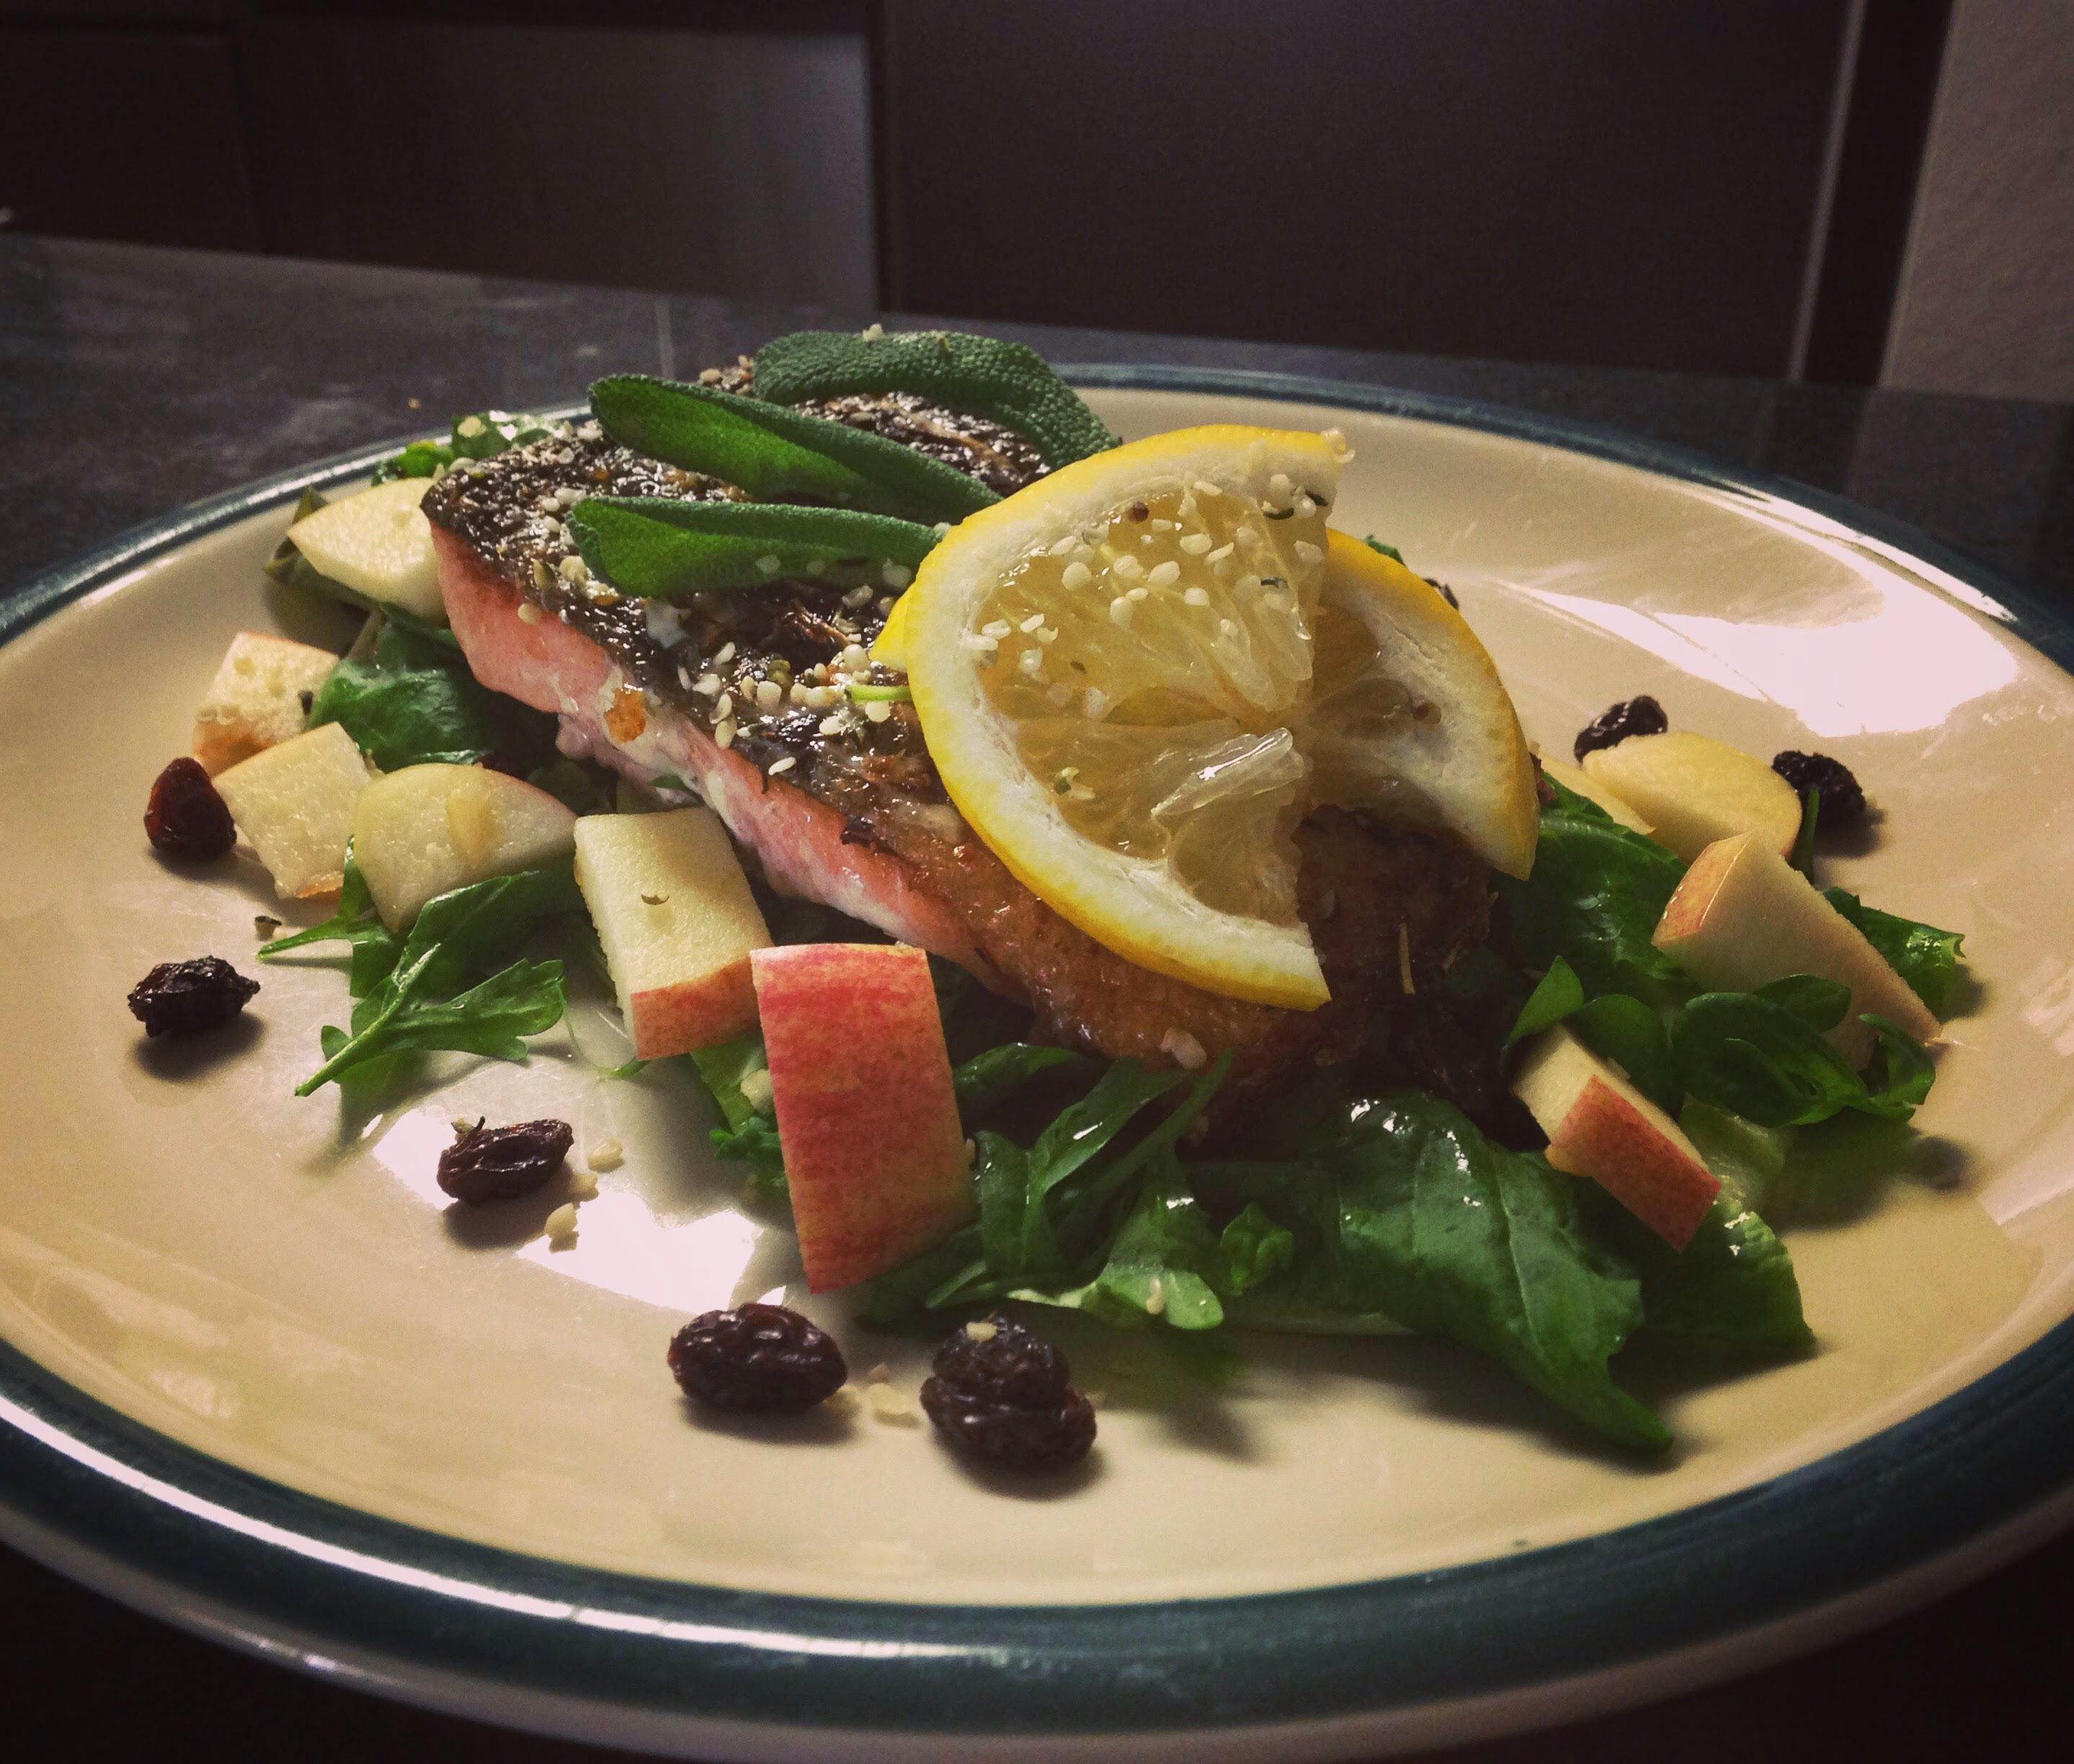
\includegraphics[height=\paperheight,%
				keepaspectratio]{./Images/SalmonSalad.jpg}}%
			\vfill
}}}

%SALMONSALAD
\newcommand\QuinoaPatties{%
	
	
	\put(0,0){%
		\parbox[b][\paperheight]{\paperwidth}{%
			\vfill
			\centering
			{\transparent{0.3} 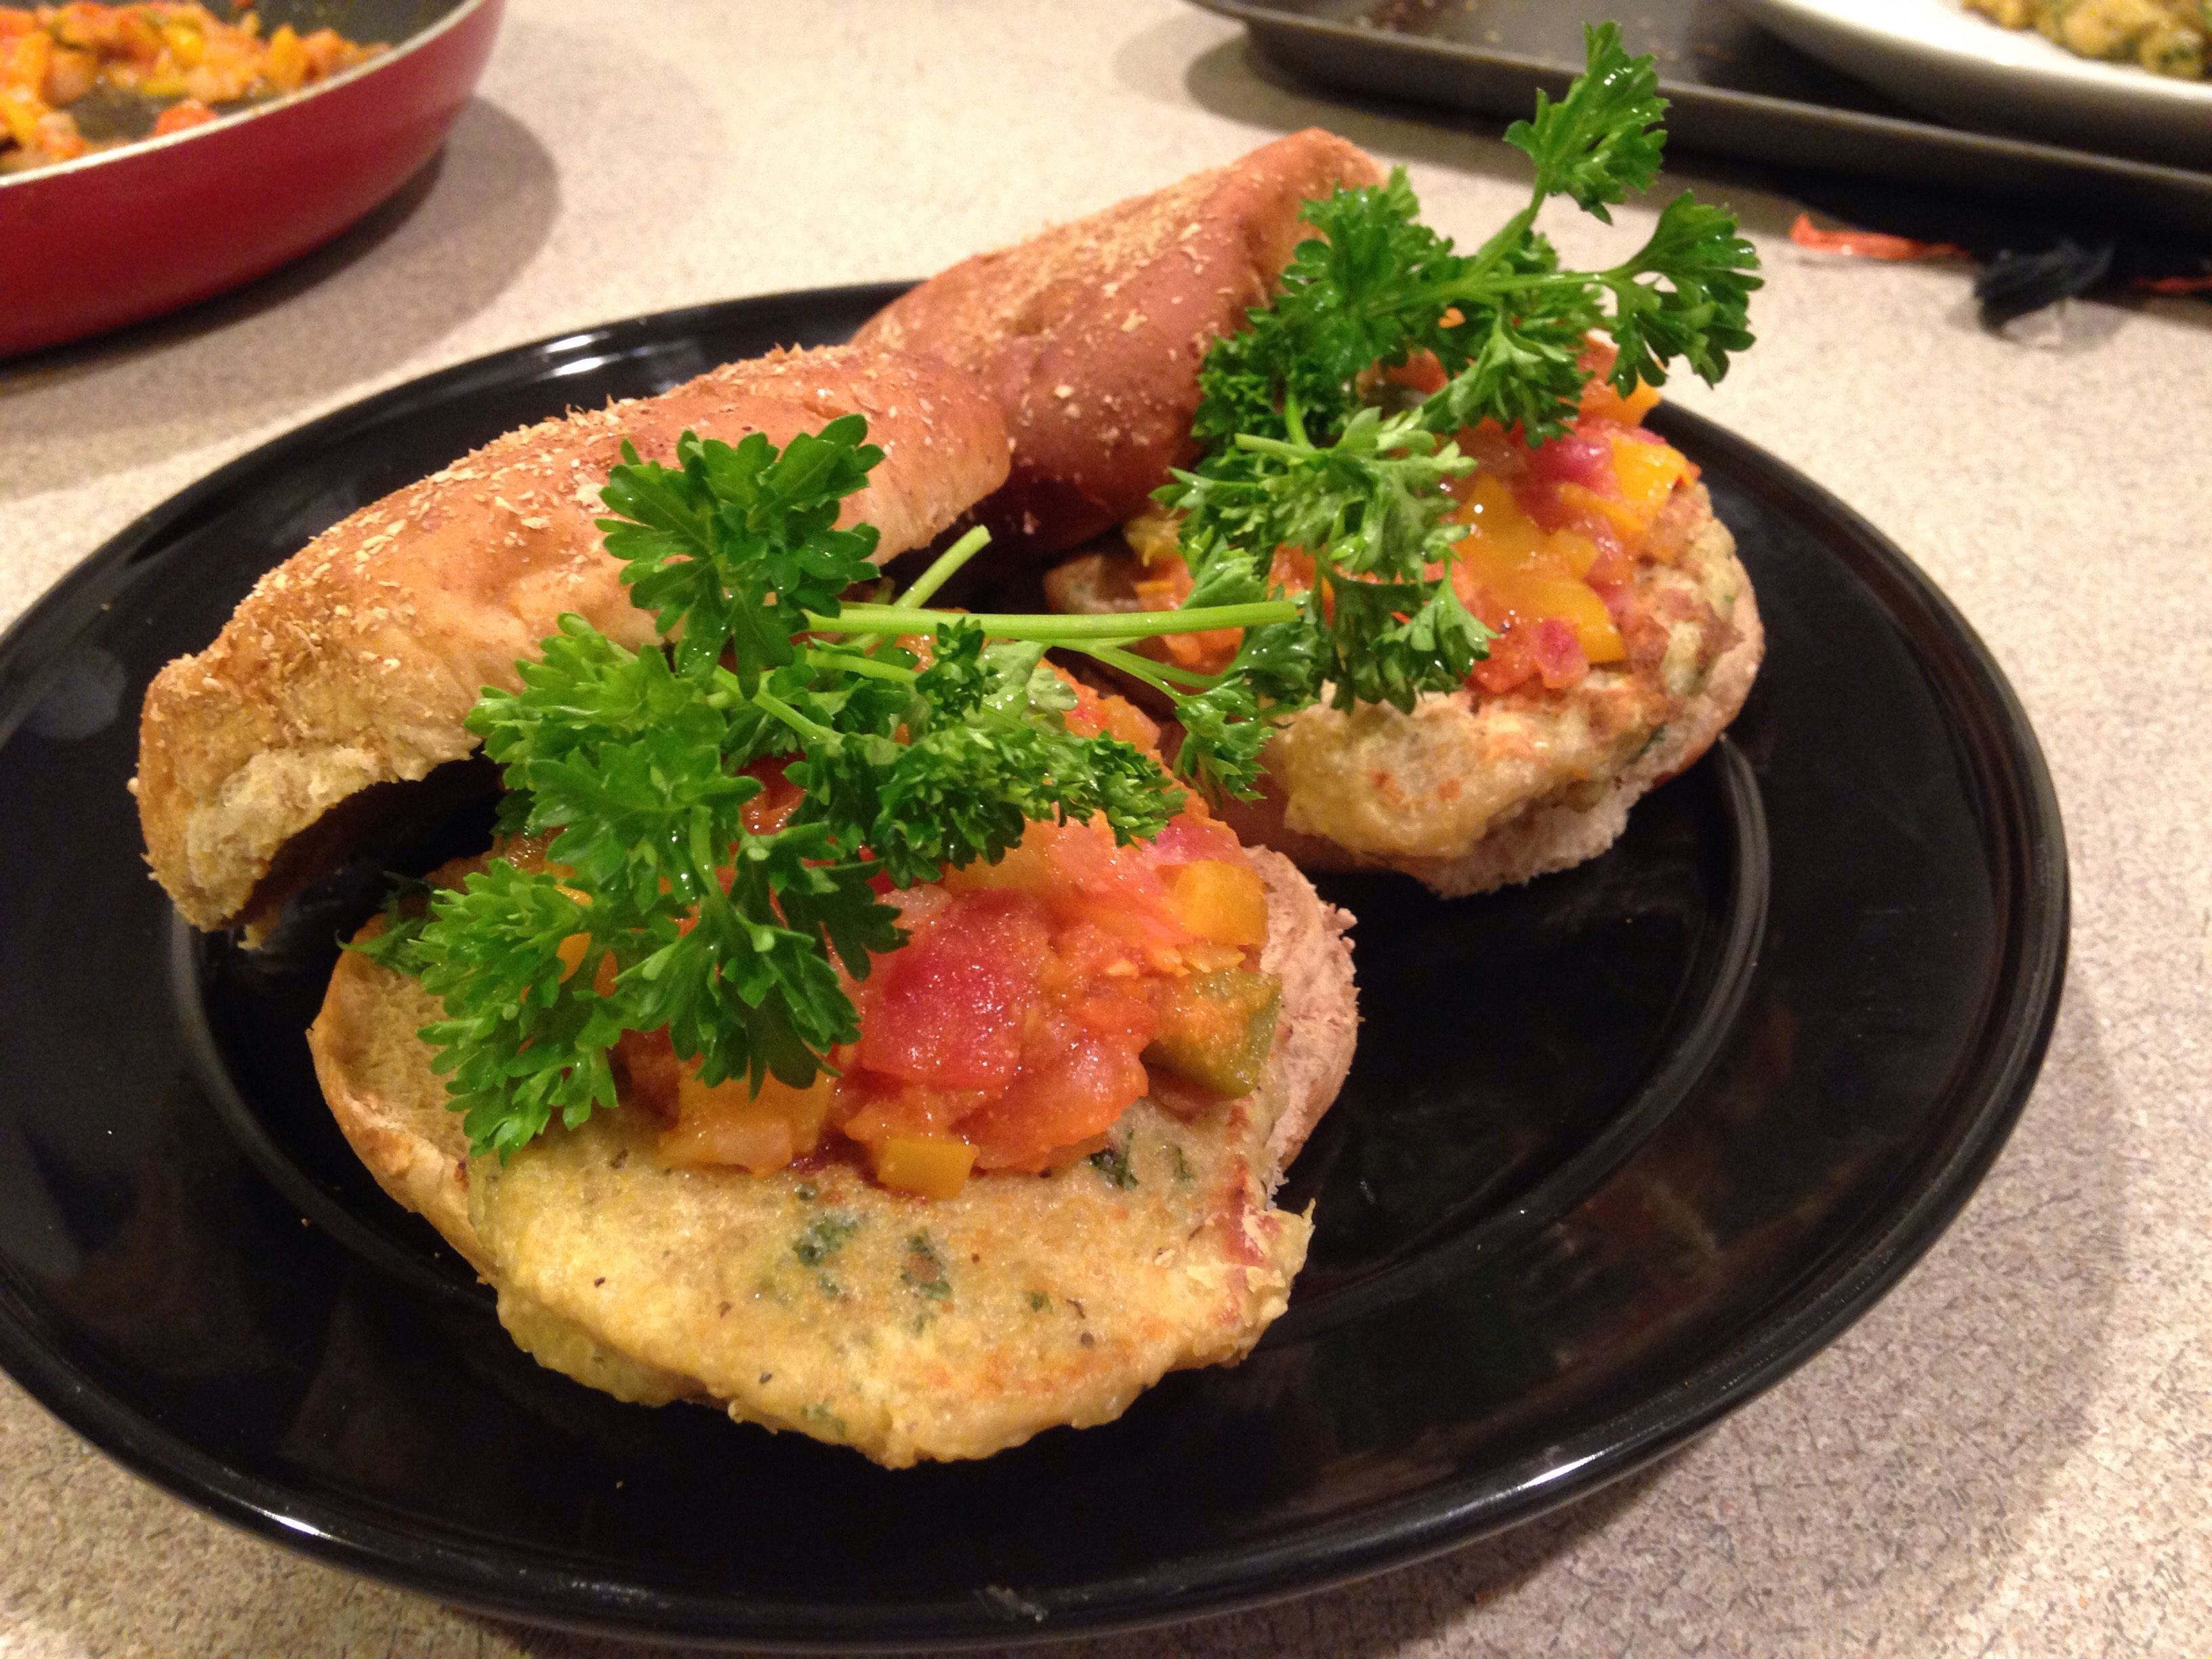
\includegraphics[height=\paperheight,%
				keepaspectratio]{./Images/QuinoaPatties.jpg}}%
			\vfill
}}}

%TITLE AND AUTHOR
\title{{\huge \textbf{Antonius' Cookbook} \\ \textbf{Version -- \Version}} \\ \vspace{1cm}
	%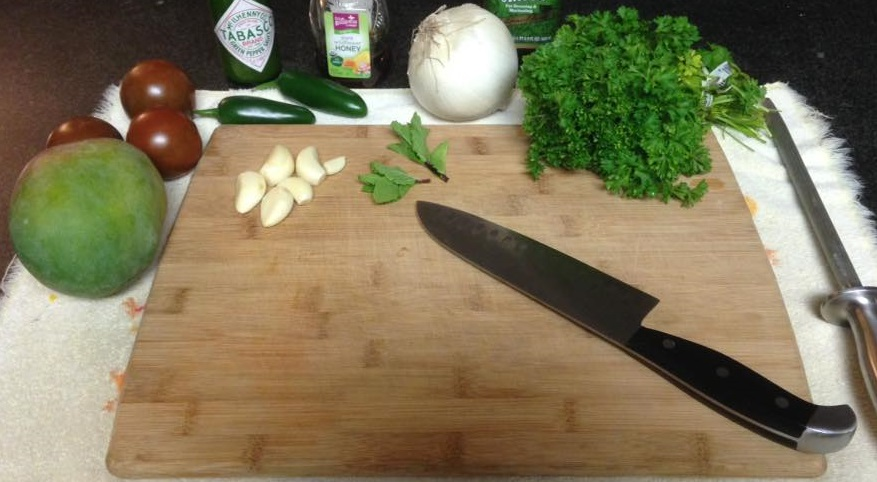
\includegraphics[scale =0.45]{./Images/CoverCropped.jpg}
}
\author{Written and Compiled by: Antonius Torode \\ Michigan State University \\ Department of Physics \& Astronomy}
\date{Latest update: \today}

\begin{document}
	
\AddToShipoutPicture*{\CoverPic}

%BEGIN FRONT MATTER
\setlength{\parindent}{0pt}
\frontmatter
\clearpage
\maketitle
\pagestyle{empty}
\AddToShipoutPicture*{\TowerGarden}
%% copyrightpage
\begingroup
\footnotesize
\parindent 0pt
\parskip \baselineskip
\textcopyright{} 2017 Antonius Torode \\
All rights reserved.

This work may be distributed and/or modified under the conditions of Antonius’ General Purpose License (AGPL).

The Original Maintainer of this work is: Antonius Torode.

The Current Maintainer of this work is: Antonius Torode.

Primary Shareholder: Pranjal Tiwari

This document is designed for the purpose of storing and sharing recipes that have either been discovered by or created by myself (the author). All images are taken by myself of meals I have prepared unless otherwise stated.

\begin{center}
\begin{tabular}{ll}
Most Current Revision Date: &  \today 
\end{tabular}
\end{center}

Published by Antonius Torode. 

Hosted at: https://msu.edu/{\raise.17ex\hbox{$\scriptstyle\sim$}}torodean/ACookbook.html

Github Repository: https://github.com/torodean/Antonius-Cookbook

\vfill


Torode, A.\\
\hspace*{2em} The Antonius Cookbook \\
\hspace*{2em} Version -- \Version \\
\hspace*{2em} Michigan State University -- \\
\hspace*{2em} Department of Physics \& Astronomy. \\
\hspace*{2em} 2016, Student. \\
\hspace*{2em} ISBN: NONE \\



\endgroup
\clearpage
\tableofcontents
\newpage
\vspace*{\fill}
\begin{center}
	\textit{This page intentionally left blank. \\ (Yes, this is a contradiction.)}
\end{center}
\vspace*{\fill}

%BEGIN MAIN MATTER
\mainmatter
\pagestyle{fancy}
\chapter{Breakfasts}
	
\thispagestyle{fancy}
\section{Egg Sandwich}
\AddToShipoutPicture*{\EggSandwich}

\subsection*{Base Ingredients}
\begin{multicols}{3}
	\begin{itemize}
		\item English Muffin or Toast
		\item 2-3 Eggs
		\item Beef Summer Sausage
		\item Butter
		\item Olive oil
		\item Milk
		\item Garlic
		\item Salt \& Pepper
	\end{itemize}
\end{multicols}
\subsection*{Spinach and Feta (optional)}
\begin{multicols}{3}
	\begin{itemize}
		\item Spinach
		\item Feta Cheese
		\item Onion
	\end{itemize}
\end{multicols}
\subsection*{Greek Delight (optional)}
\begin{multicols}{3}
	\begin{itemize}
		\item Mushroom
		\item Green Pepper
		\item Onion
		\item Tomato
		\item Ginger
		\item Fresh Parsley
	\end{itemize}
\end{multicols}

\subsection*{Your Favorite Omelet}
You can use ingredients of your liking. This is a very versatile dish.

\subsection*{Preparation}
Toast English muffin or bread to desired level while preparing other ingredients. Scramble eggs in a separate bowl with a small drizzle of milk (this helps them fluff up) and dice other optional ingredients. Slice Summer Sausage into circles and place in a medium-low heat pan. When the sausages start to bubble, they are ready to be flipped. While that is cooking, in a hot pan, lightly drizzle olive oil and place in Minced Garlic and other optional ingredients\footnote{If you are using greens such as spinach, parsley, cilantro, etc. or cheeses such as cheddar, swiss, feta, etc., wait to put these in until the eggs are in.}. Saut\`{e} these until they start browning. Once browning begins, add eggs\footnote{This is when it is a good idea to add items such as Parsley, Spinach, cheese, etc.}. Place lobs of butter on edges of omelet as it cooks. Once cooked, add Salt \& Pepper and remove from pan. 

When toast is finished, butter it. When sausage is finished, dab with paper towel to remove excess grease. Cut omelet in half or appropriate size for bread and assemble sandwich by bread|egg|sausage|bread. Enjoy with a side of fruit and a warm cup of tea for best breakfast results.


\subsection*{Tips}

Do not season the eggs before they are cooked. To practice flipping an omelet, you can get a piece of toast in an empty frying pan and flip it. A great way to slice spinach for use in something like this where you are not cooking it down for a while is to roll the leaves together and slice into strips (being careful not to crush the leaves). You can also make home made sausage with ground beef and the appropriate seasonings which will go brilliantly well as a replacement to any sausage. A small amount of fresh ginger is a great addition to most combinations of ingredients here. Cinnamon toast is also a great choice (and a childhood favorite of mine) for use with these sandwiches.

\chapter{Lunches}
\thispagestyle{fancy}
\section{Spicy Mexican Soup}
\AddToShipoutPicture*{\MexicanSoup}
This recipe was adapted from the youtube video ``Spicy Mexican Soup with Tortillas \& Salsa - Gordon Ramsay.'' I would highly recommend watching 
\subsection*{Ingredients}
\begin{multicols}{3}
	\begin{itemize}
		\item Red Onions
		\item Habanero (or chipotle)
		\item 1 Teaspoon Cumin seeds
		\item 1 Teaspoon Oregano
		\item 2 Clove Garlic
		\item Olive Oil
		\item 1 Tablespoom Brown Sugar
		\item 1 Tablespoon Tamato Puree
		\item 1 Tomato
		\item 1 Can of Kidney Beans
		\item 1 Orange Bell Pepper
		\item $\frac{1}{2}$-1 cup vegetable stock
		\item Cilantro or Coriander
	\end{itemize}
\end{multicols}

\subsection*{Preparation}

Begin by drizzling olive oil in a hit pot and add finely sliced red onions, Bell pepper and habanero. Add finely diced garlic, oregano and cumin seems and reduce down until ingredients brown. Drizzle olive oil again generously which will help reduce spice. Add brown sugar and coat ingredients in the light caramel. Add tomato puree and blend well. Add one whole diced tomato, kidney beans, and vegetable stock. Let simmer and stir occasionally. The longer you cook the dish the hotter (spicier) it will become. When done, add fresh cilantro or Coriander and mix in. 

This dish is well served with avocado and cheese or with a side of garlic bread. Garlic bread can be made simply by buttering your favorite bread, adding garlic powder and sea salt, and then baking until golden brown and crispy. 

\subsection*{Tips}

Habanero works well with this dish if you can handle a good deal of spice. If not, you may want to use something less potent like chipotle or chili peppers. You can also leave the spice out entirely but the flavor from the spice adds a lot to this dish.
\section{Mango Salsa Taco}
\AddToShipoutPicture*{\MangoSalsaTaco}

\chapter{Dinners}
\thispagestyle{fancy}
\section{Calzone}
\AddToShipoutPicture*{\Calzone}

\subsection*{Ingredients}

\chapter{Deserts}
\thispagestyle{fancy}
\section{New York Cheesecake}
\AddToShipoutPicture*{\Cheesecake}
\thispagestyle{fancy}
\section{Cheesecake Topping}
\AddToShipoutPicture*{\CheesecakeTopping}

\subsection*{Ingredients}

%BEGIN BACKMATTER
\backmatter
% bibliography, glossary and index would go here.

\end{document}